\chapter{Network Layer}
\label{chapter:networklayer}

This section explains the network layer and describes how its responsiblites were designed and implemented.

The network layer is the bottom layer in the 3 layer architecture of ACE. The network layer is responsible for all communication issues between running instances of ACE that are connected by communication networks. The core responsiblities are:

\begin{itemize}
 \item automatic user discovery in the local area network
 \item explicit user discovery on the Internet
 \item document management communication
 \item collaborative editing session communication
\end{itemize}

The network layer can be viewed as the interface between the physical network and the collaboration layer. Therefore, all messages received from the physical network are appropriately processed and passed to the collaboration layer. The network layer is not aware of the application layer.

Basically, the network layer provides core functionality independent of the activity of the user. Besides, depending on the activity of the user, being either participant or publisher of a document session, the network layer provides a client specific part (participant part) and a server specific part (publisher part).


\section{Overview}

This section gives a high-level overview about the network layer design and implementation by using two different points of view.

\subsection{Architecture}

The figure \ref{fig:network.architecture} depicts the rough architecture of the network layer. The collaboration layer interacts only with the \texttt{Net} component. Through this component, the collaboration layer either accesses the \texttt{Protocol} component or the \texttt{Core} component. The latter interacts with the \texttt{Discovery} component as well as with the \texttt{Protocol} component. The \texttt{Protocol} accesses the \texttt{BEEP} framework whereas the \texttt{Discovery} accesses the \texttt{DNSSD} (Bonjour) service.

\begin{figure}[H]
 \centering
 \frame{
 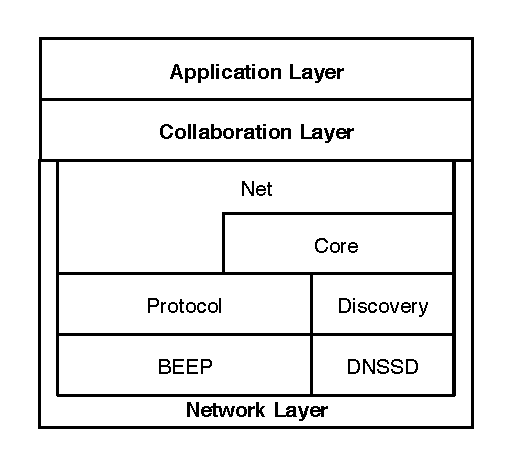
\includegraphics[width=3.19in,height=2.89in]{../images/finalreport/network_architecture_view.eps}
 }
 \caption{Network Layer Architecture}
 \label{fig:network.architecture}
\end{figure}


\subsection{Packages}

The top level package \texttt{net} contains all the interfaces through which the collaboration layer and the network layer interact. All other packages in the network layer are subpackages of the \texttt{net} package. The \texttt{core} package provides core classes to the network layer and contains default implementations for several interfaces declared in the \texttt{net} package. It depends on the \texttt{protocol} and the \texttt{discovery} packages.

The \texttt{discovery} package contains the relevant functionality for dynamic user discovery as well as user management. It has a subpackage \texttt{dnssd} which contains DNSSD specific classes (compare appendix \ref{chapter:frameworks.bonjour}). The \texttt{discovery} and the \texttt{dnssd} packages interact with the DNSSD component.

The \texttt{protocol} package implements all communication related functionality and directly interacts with the BEEP component. The subpackage \texttt{filter} contains classes for the processing of outgoing and incoming requests and messages, respectively (see section \ref{chapter:networkfilterchains}).

\begin{figure}[H]
 \centering
  \frame{
 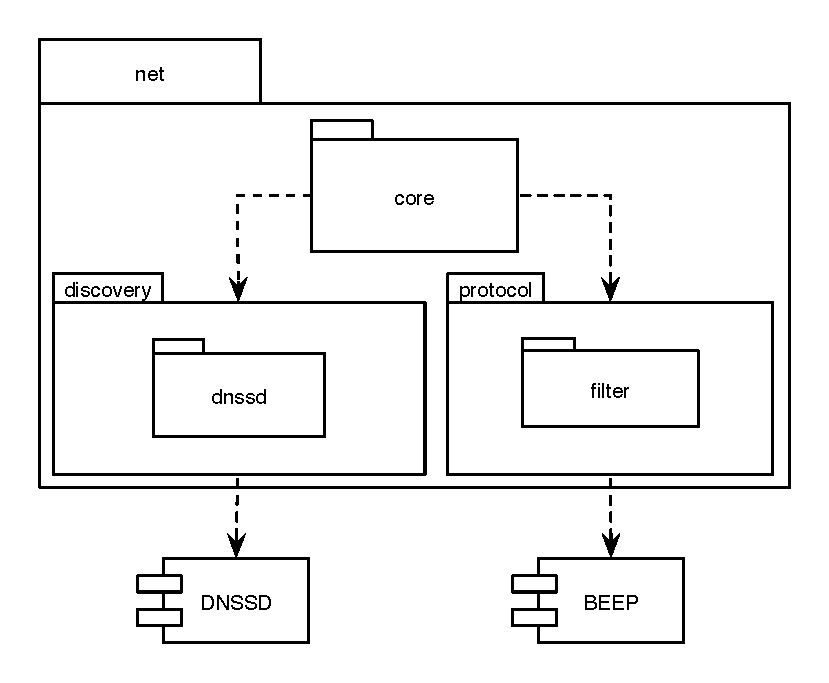
\includegraphics[width=4.80in,height=3.91in]{../images/finalreport/network_package_view.eps}
 }
 \caption{Network Layer Package Structure}
 \label{fig:network.architecture.package}
\end{figure}


\section{User Discovery component}
This section explains the design and the implemented solution for the dynamic and automatic user discovery in greater detail.

\subsection{Responsabilities}
The user discovery takes over the task of discovering all possible events in the local area network that are interesting for the user. This includes the dynamic discovery of new users, the leaving of users and the notification of metadata changes for a particular user. Currently, a user's changeable metadata is currently only the nickname of a user, i.e. a user can change his nickname and all other peers get notified through the discovery mechanism.

The user discovery component must meet the following core requirements:

\begin{itemize}
 \item notification about new discovered users
 \item deliver full address information for each discovered user
 \item notification about discarded users
 \item notification about user detail changes
 \item start and stop possiblity for the discovery process 
\end{itemize}

These requirements could be met by multiple technologies. We decided that Bonjour zero-conf networking technology would best meet our requirements. Please read the chapter \ref{chapter:decisionsnetwork} for a justification of that decision.

\subsection{Design}
\subsubsection{Client view of the discovery component}
The first step in the design of the discovery component was to find a way to use the discovery component independently of its implementation. That is, to have a transparent discovery usage for the client, without him knowing the concrete implementation. This consideration is in line with the general design principle of ACE to have an architecture with interchangeable components.

\begin{figure}[H]
 \centering
  \frame{
 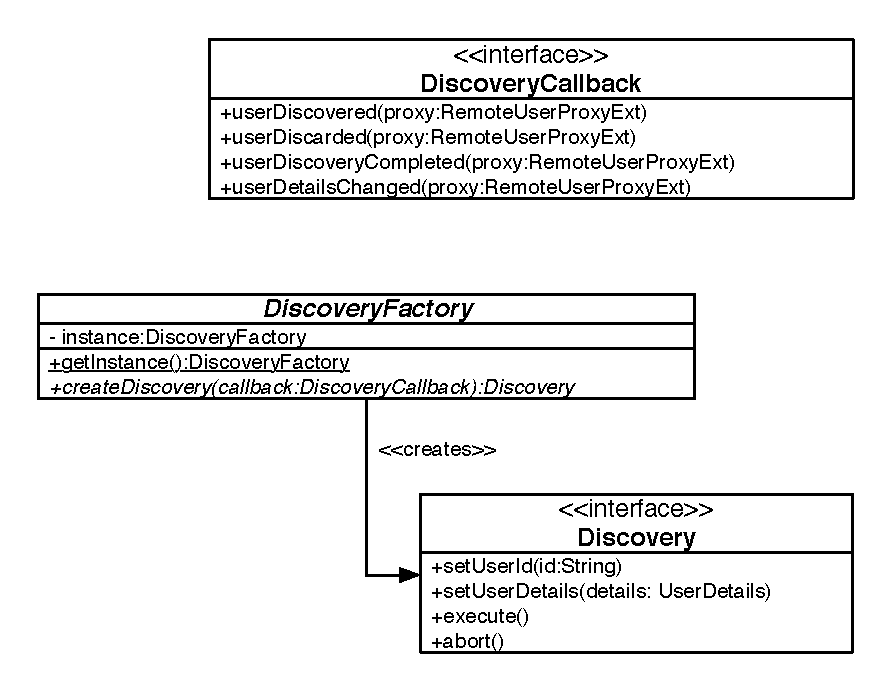
\includegraphics[width=5.72in,height=4.39in]{../images/finalreport/network_discovery_uml.eps}
 }
 \caption{Discovery usage design}
 \label{fig:network.discovery.usage}
\end{figure}

The abstract class  \texttt{DiscoveryFactory} provides the entry point for a client who wants to use the discovery service. To create a new  \texttt{Discovery}, a  \texttt{DiscoveryCallback} implementation must be passed. This implementation is provided by the client to the \texttt{Discovery}. All events received from the network by the discovery are finally forwarded to that callback object. The  \texttt{Discovery} interface enables the client to set the  essential information for the local user and to start and stop the discovery service.

This design makes the concrete discovery implementation (i.e. the technology used) transparent to the client.


\subsubsection{DiscoveryManager}
The  \texttt{DiscoveryManager} plays a major role in the discovery component. It keeps track of all active users (who have not been discarded) and their session states (established/not established). All user management is done through this class. So each other component of the network layer falls back on the  \texttt{DiscoveryManager} if user bookkeeping is needed.

All events that the discovery receives are first processed in collaboration with the \texttt{DiscoveryManager} implementation (compare also interface \texttt{DiscoveryCallbackAdapter}) before they are passed to the  \texttt{DiscoveryCallback}.

\begin{figure}[H]
 \centering
  \frame{
 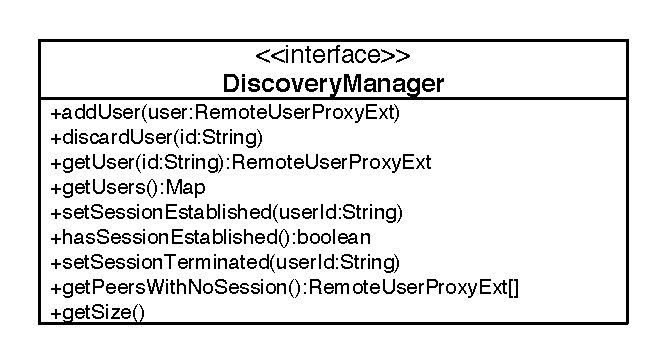
\includegraphics[width=4.22in,height=2.19in]{../images/finalreport/network_discoveryManager_uml.eps}
 }
 \caption{Discovery Manager}
 \label{fig:network.discovery.manager}
\end{figure}


\subsubsection{DNSSD calls}
\label{chapter:discovery.dnssdcall.introduction}
\texttt{DNSSDCall} is an abstract base class for all DNSSD API calls. A subclass defines what API call is executed. \texttt{DNSSDCall} incorporates advanced \texttt{Exception} and \texttt{Error} handling. That is, in case of failure, it uses a \texttt{RetryStrategy} to determine how many times and in what intervals a call is repeated. Consider the design of the \texttt{execute()} method:

\begin{verbatim}
public Object execute() throws DNSSDUnavailable {
   RetryStrategy strategy = getRetryStrategy();		
   while (strategy.shouldRetry()) {
      try {
         return makeCall();
      } catch (DNSSDCallException dex) {
         try {
            strategy.exceptionOccurred();
         } catch (RetryException re) {
            throw new DNSSDUnavailable();
         }
      }
   }
   return null;
}
\end{verbatim}

Method \texttt{makeCall()} executes the actual DNSSD API call. If \texttt{makeCall()} throws a \texttt{DNSSD\-Call\-Exception}, the retry strategy is notified that an exception occured and if the call should be retried again. If the retry strategy fails, then it throws a \texttt{RetryException}. In turn, method \texttt{execute()} throws a \texttt{DNSSD\-Unavailable} exception up the call stack. 
The \texttt{DNSSDCall} design follows the command pattern (see [Design Patterns]) in that each call is wrapped by a command object and can be executed uniformly through the method \texttt{execute()}.



\begin{figure}[H]
 \centering
  \frame{
 
\includegraphics[width=2.97in,height=1.08in]{../images/finalreport/network_dnssdCall_uml.eps}
 }
 \caption{DNSSDCall abstract super class}
 \label{fig:network.discovery.dnssdCall}
\end{figure}


\subsection{Implementation}
This section outlines how the concrete discovery implementation with Bonjour was designed and implemented. The design was lead by the listener oriented API of Bonjour (see \ref{chapter:frameworks.bonjour} for further details on this technology).

\subsubsection{Bonjour discovery}
The concrete \texttt{Discovery} implementation is called \texttt{Bonjour} and is created by the \texttt{BonjourFactory} factory. Class \texttt{Bonjour} starts and stops the discovery process with Bonjour zero-conf networking technology. For this purpose,  \texttt{Bonjour} makes use of two further types:  \texttt{UserRegistration} and \texttt{PeerDiscovery}.

\begin{figure}[H]
 \centering
  \frame{
 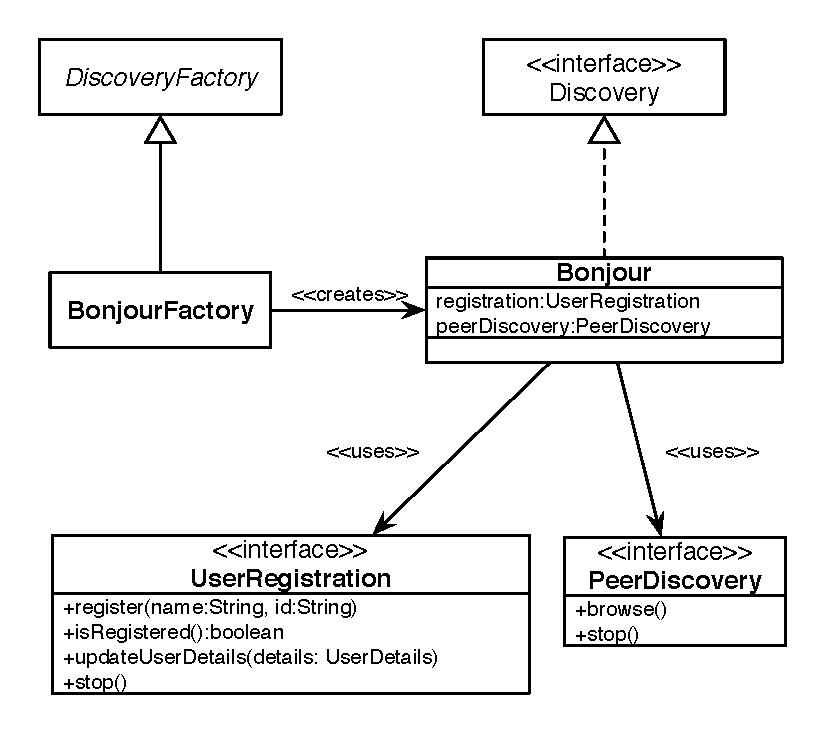
\includegraphics[width=5.28in,height=4.67in]{../images/finalreport/network_bonjour_uml.eps}
 }
 \caption{Discovery Implementation}
 \label{fig:network.discovery.implementation}
\end{figure}

\paragraph{User Registration}
 \texttt{UserRegistration} allows to register the local user for discovery as well as to update the user's details. It extends 
 various listener interfaces specified by the DNSSD API, namely  \texttt{RegisterListener},  \texttt{ResolveListener} and  \texttt{QueryListener}. This allows to have the user registration process separate from the peer discovery process, which uses the same listener interfaces. Consider figure \ref{fig:network.discovery.userregistration}.

\begin{figure}[H]
 \centering
  \frame{
 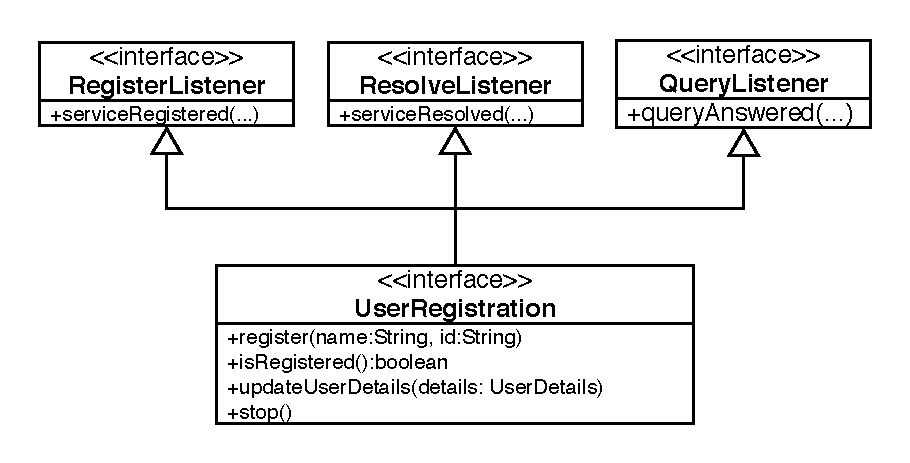
\includegraphics[width=5.85in,height=2.86in]{../images/finalreport/network_userRegistration_uml.eps}
 }
 \caption{User Registration and extended interfaces}
 \label{fig:network.discovery.userregistration}
\end{figure}


\paragraph{Peer Discovery}
\begin{figure}[H]
 \centering
  \frame{
 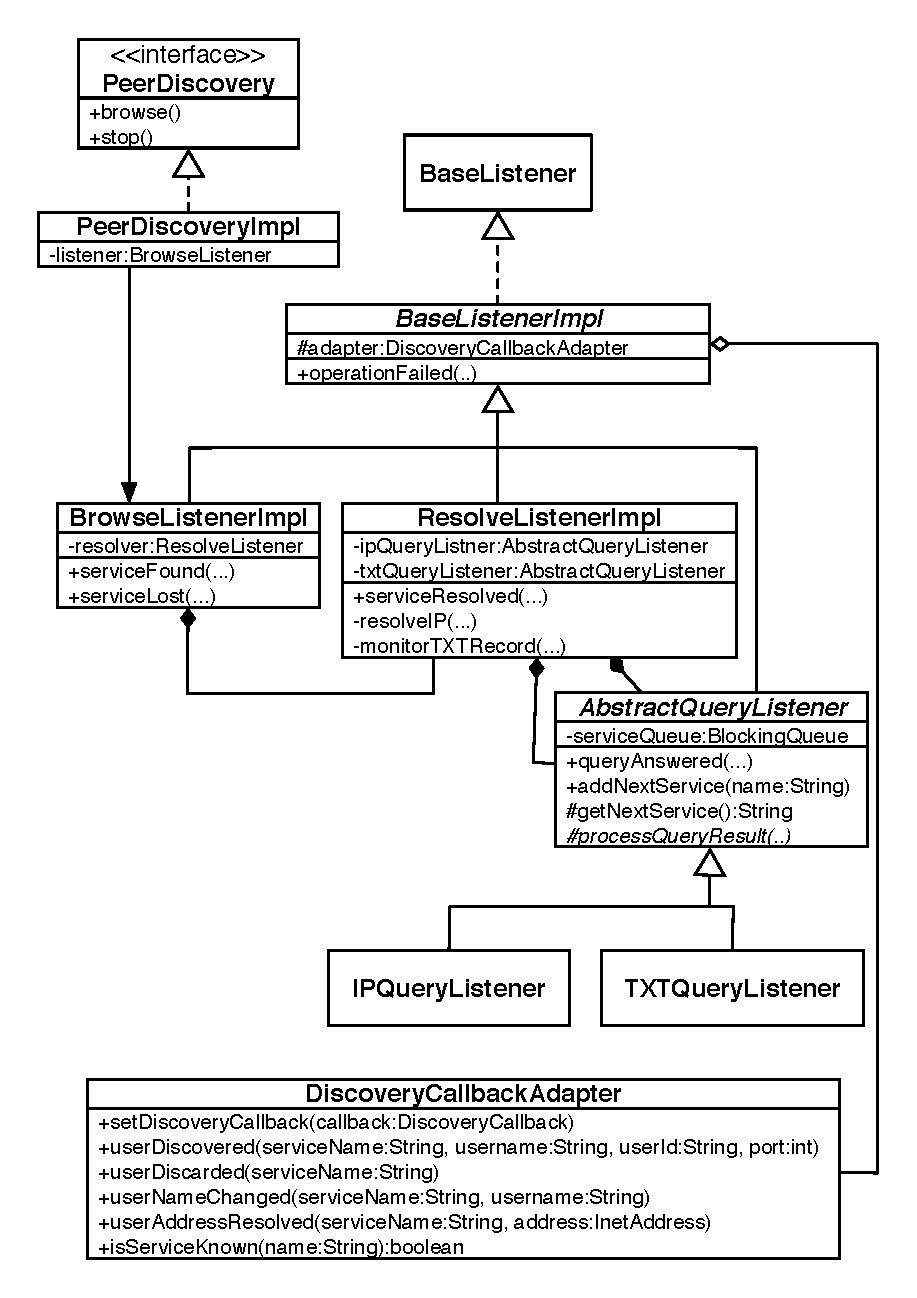
\includegraphics[width=5.89in,height=8.43in]{../images/finalreport/network_peerDiscovery_uml.eps}
 }
 \caption{Peer Discovery Design and Implementation}
 \label{fig:network.discovery.peerdiscovery}
\end{figure}

\texttt{PeerDiscovery} allows for the discovery of peer users who reside on the same local area network (this constraint is   imposed by the Bonjour technology). The \texttt{PeerDiscovery} implementation has a reference to the \texttt{BrowseListenerImpl} class. It receives browse events from the DNSSD component (\emph{serviceFound}, \emph{serviceLost}). When a new service (i.e. user) was found, \texttt{BrowseListenerImpl} starts a new DNSSD call to resolve that service (i.e. receive TXT record with specific information for that user). The call is passed a reference to \texttt{ResolveListenerImpl}, which will receive the results of that call (see also section \ref{chapter:network.discovery.dnssdcalls} on DNSSD calls). On the other side, a \emph{serviceLost} event is directly forwarded to the \texttt{DiscoveryCallbackAdapter} (see below for a description of that class). 

\texttt{ResolveListenerImpl} handles \emph{serviceResolved} events. It first forwards the event to the \texttt{DiscoveryCallbackAdapter} and second starts two further DNSSD calls for resolving the IP address of the discovered user and monitoring for the user's TXT record (i.e. to be notified when that user changes its TXT record, e.g. his name).

The listeners for the two DNSSD calls are \texttt{IPQueryListener} and \texttt{TXTRecordListener}. Both extend the \texttt{AbstractQueryListener}. Their functionality is straightforward: The events are simply forwarded to the \texttt{DiscoveryCallbackAdapter}.

The \texttt{DiscoveryCallbackAdapter}, as its name suggets, is an adapter for all listeners to forward their DNSSD events. This class allows to have a central place where all events from the DNSSD discovery are gathered and uniformly processed. The implementation of this interface \texttt{DiscoveryManagerImpl} also implements \texttt{DiscoveryManager} and represents the central processing place for events from the discovery side as well as the user management handler for the remaining network layer part.

\begin{figure}[H]
 \centering
  \frame{
 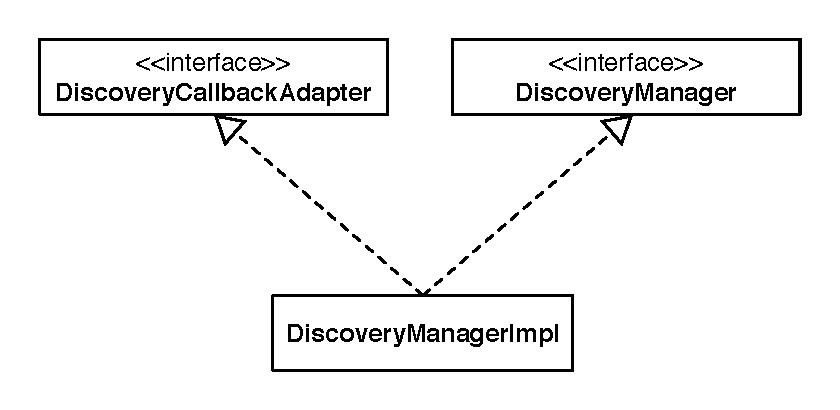
\includegraphics[width=5.38in,height=2.51in]{../images/finalreport/network_discoveryManagerImpl_uml.eps}
 }
 \caption{Discovery Callback Adapter and Discovery Manager Implementation}
 \label{fig:network.discovery.managerandadapter}
\end{figure}


\paragraph{Concrete DNSSD calls}
\label{chapter:network.discovery.dnssdcalls}
There are various implementations for the abstract super class \texttt{DNSSDCall}, including \texttt{Register}, \texttt{Browse}, \texttt{Resolve}, \texttt{QueryRecord} and \texttt{TXTUpdate}. Each of these commands wraps the respective DNSSD API call. If a call throws a \texttt{DNSSDUnavailable} exception (after the retry strategy failed), then the exception is reported to the upper layer (trough \texttt{NetworkServiceCallback}) and the discovery process aborted (See section \ref{chapter:network.exceptionhandling} for further details).

\begin{figure}[H]
 \centering
  \frame{
 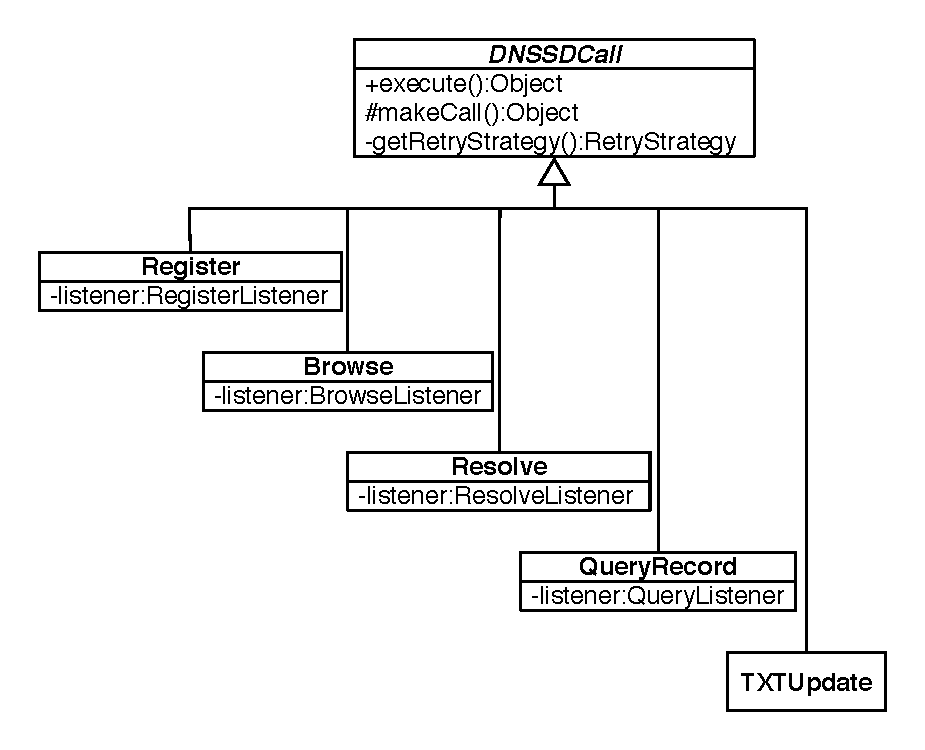
\includegraphics[width=5.94in,height=4.78in]{../images/finalreport/network_dnssdCall_impl_uml.eps}
 }
 \caption{DNSSDCall implementations}
 \label{fig:network.discovery.dnssdCall.impl}
\end{figure}


\subsection{TXT record protocol}
The TXT record gives a service the chance to publish some metadata such as the service version and id. ACE uses a simple TXT record protocol which contains the following information:

\begin{itemize}
\item the user name
\item the user id
\item the communication protocol version
\item TXT record protocol version (standard)
\end{itemize}

The content of an example TXT record would look like: \\
\texttt{0=\{txtvers=1\}, 1=\{name=Lukas' Dell\}, 2=\{userid=805f9e71-5f68-4d51-ab96-24d3dcca6651\}, 3=\{version=1.0\}}.\\The user name may be updated whereas the other values remain constant. The protocol version could be used in case of a new protocol version to detect incompatibilities.

\subsection{Explicit user discovery}
The explicit discovery of a user is not related to the discovery component. Therefore read section \ref{chapter:network.protocol.explicituserdiscovery} in the protocol chapter.

\subsection{Use cases}
\subsubsection{Start of discovery process}
The following sequence diagram shows how the client uses the discovery and what happens behind the \texttt{Discovery.execute()} call.

\begin{figure}[H]
 \centering
  \frame{
 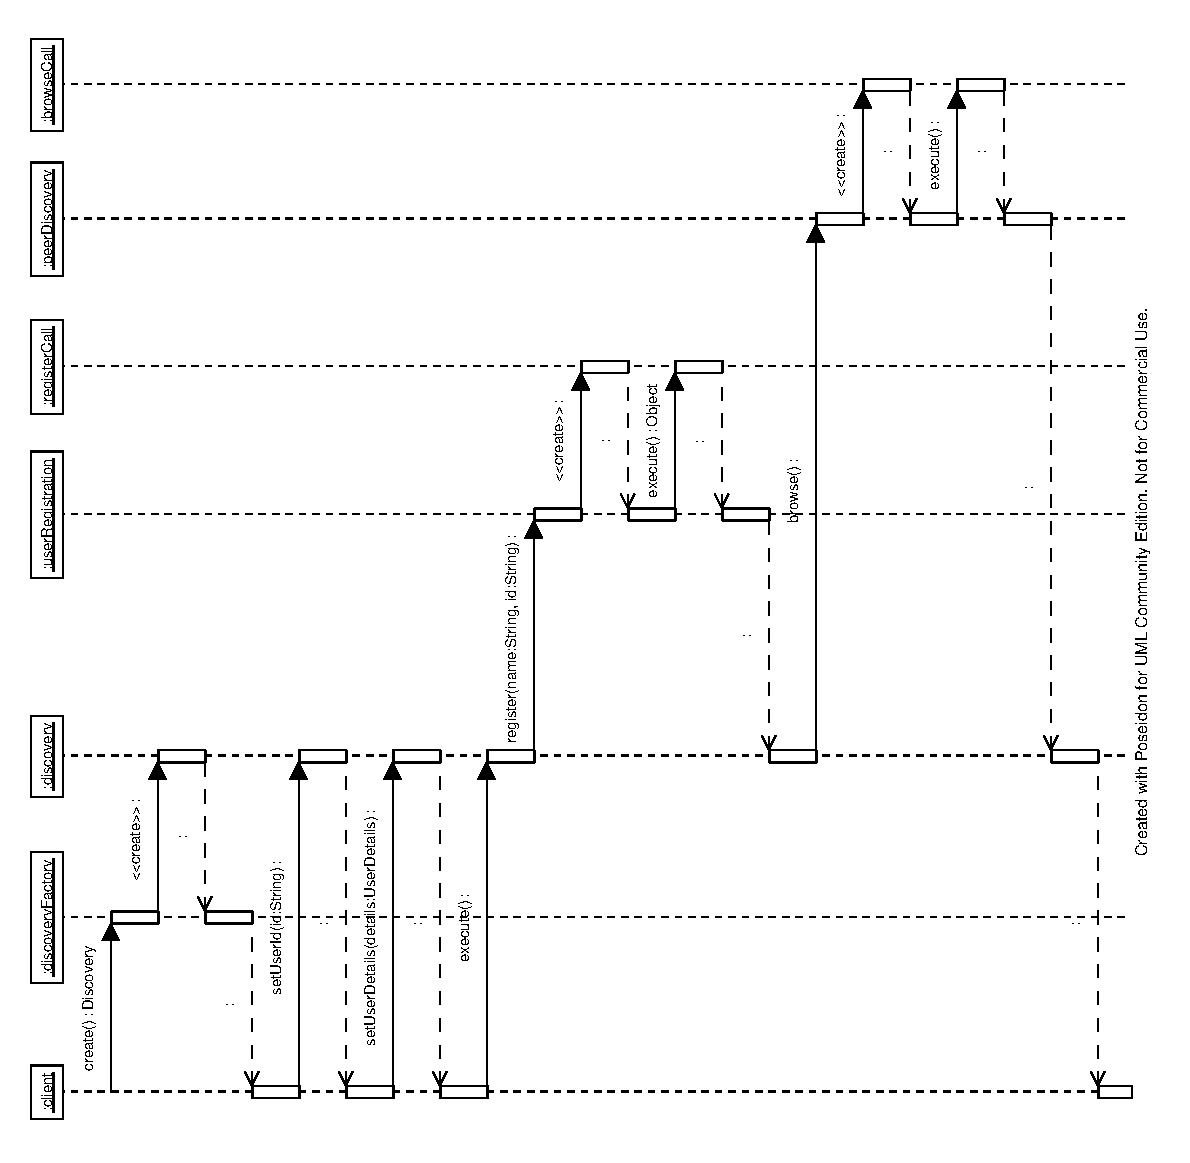
\includegraphics[width=5.90in,height=5.76in,angle=-90]{../images/finalreport/network_discovery_sequence.eps}
 }
 \caption{Launch of the Discovery Process}
 \label{fig:network.discovery.launch}
\end{figure}


\subsection{Exception handling}
All necessary exception handling for the discovery component is captured in \texttt{DNSSDCall} and in \texttt{BaseListenerImpl}. See section \ref{chapter:discovery.dnssdcall.introduction} for a description of the exception handling implemented in \texttt{DNSSDCall}.

If the first executed DNSSD call throws an \texttt{Error} (usually \texttt{UnsatisifedLinkError}), then this is interpreted that the DNSSD (Bonjour) is not installed on the local host. The discovery process is aborted and the upper layer notified.

\texttt{BaseListenerImpl} implements an exception method \texttt{operationFailed(...)} which must be available for all DNSSD listeners. If this method is called, it is interpreted as an unrecoverable error. Thus, the upper layer gets reported and the discovery process aborted.

\subsubsection{Retry Strategy}
The retry strategy design shall give an advanced exception handling and some way of service recovery in that calls are retried a certain number of times. The retry strategy determines how long the executing thread should wait untill it retries to execute the DNSSD call. If the call fails again, the retry strategy is asked again how long the thread should wait untill the next call. This algorithm may repeat over and over depending on the retry strategy implementation. If the retry strategy fails, it throws a \texttt{RetryException} to indicate that the thread should stop retrying the DNSSD call and abort. This strategy could be applied for all network related method calls, but yet it is used only for DNSSD calls. 

\begin{figure}[H]
 \centering
  \frame{
 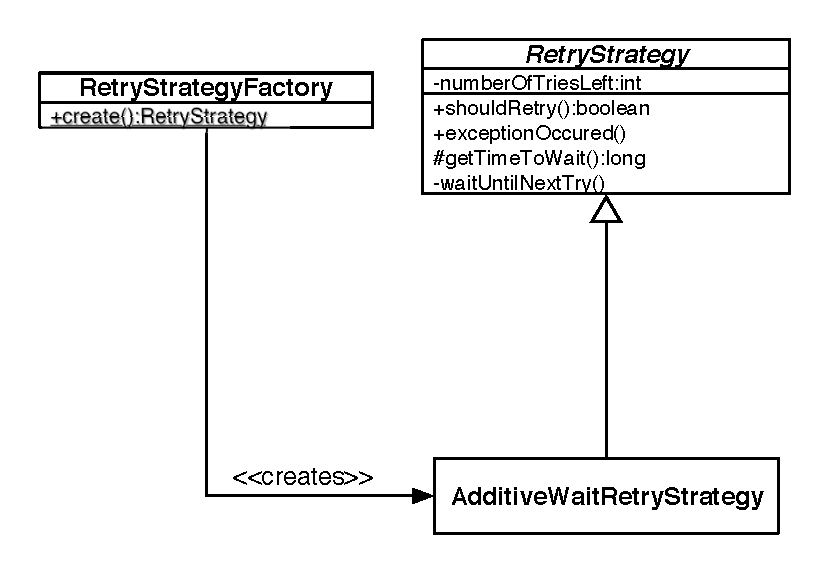
\includegraphics[width=5.31in,height=3.60in]{../images/finalreport/network_retryStrategy_uml.eps}
 }
 \caption{Retry Strategy Design and Implementation}
 \label{fig:network.discovery.retrystrategy}
\end{figure}

The \texttt{AdditiveWaitRetryStrategy} can be configured to start with an initial waiting time and an increment wait time for succeeding retries. So for example, if the initial waiting time is 3 seconds and the increment wait time is 2 seconds, the executing thread of the DNSSD call will wait for 3 seconds after the first failed execution of the call, and 5 seconds after the second time and so on untill the strategy throws a \texttt{RetryException} indicating that the thread should abort retrying.

% end documentation of user discovery

\newpage

\section{Communication component}
This section describes the design and the implementation of the communication component in greater detail. Henceforth, a basic knowledge of the Java BEEP Core library is expected in order to understand the explanations. See section \ref{chapter:framework.beepcore} for an introduction on BEEP Core.

\subsection{Responsabilities}
The communcation component is responsible for all communication between the peers and users, respectively. Communication includes messages for document management (publish a document, invite a user, etc.) and the collaborative editing session (caret updates, operation messages, etc.). These messages must be processed, i.e. serialized and deserialized and handled appropriately. Each discovered user and his shared documents must be managed. 
Apart from that, the communication component must manage network connections to other users and provide a fair exception handling.

In summary, the communication component must meet the following requirements:

\begin{itemize}
 \item Enable communication to and from each available peer
 \item Document management for each available peer
 \item Appropriate processing of received messages and reporting them to the upper layer
 \item Fair error reporting to the upper layer
\end{itemize}

These requirements can be categorized as follows:

\begin{itemize}
 \item Published Documents Management
 \item Remote User and Shared Documents Management
 \item Network Connection Management
 \item Network Message Processing
 \item (Collaborative Editing) Session Management
\end{itemize}

These categories are expanded thorougly in section \ref{network.communication.implementation}. Concepts used to implement the requirements are explained next.

\subsection{Design and Concepts}
This section explains the concepts worked out for the network layer. Besides, design aspects of the implemented solutions are outlined too.

\subsubsection{Remote User and Shared Documents Management}
The user management is centered around \texttt{RemoteUserProxy}. A  \texttt{Remote\-User\-Proxy} represents a discovered and alive user. The  \texttt{DiscoveryManager} keeps a reference to all user proxies, it is therefore the central place to get the  \texttt{RemoteUserProxy} for a particular user. A user may have an arbitrary number of shared documents. Such documents are modelled by  \texttt{RemoteDocumentProxy}. A  \texttt{RemoteDocumentProxy} contains the essential information about a shared document.

\begin{figure}[H]
 \centering
  \frame{
 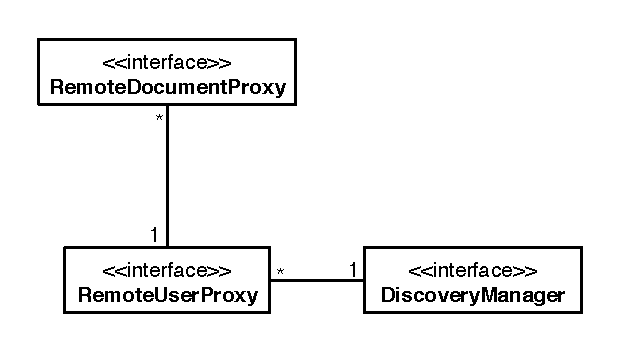
\includegraphics[width=3.92in,height=2.12in]{../images/finalreport/network_userManagement_uml.eps}
 }
 \caption{User Management}
 \label{fig:network.discovery.usermanagement}
\end{figure}

\paragraph{Interface extensions}
Types  \texttt{RemoteUserProxy}  and  \texttt{RemoteDocumentProxy} are extended for the network layer to provide an interface that allows modfications whereas the root interfaces are read-only since they are designed primarily for the upper layer.

 \texttt{RemoteUserProxyExt} adds methods mainly for document management. The methods reflect the one-to-many relationship between user and document. Besides, state methods allow to indicate if a user was discovered by DNSSD or explicitly and if a \texttt{RemoteUserSession} for the user exists. If a \texttt{RemoteUserSession} for a particular user exists, this means that a physical connection to that user has been established.

\begin{figure}[H]
 \centering
  \frame{
 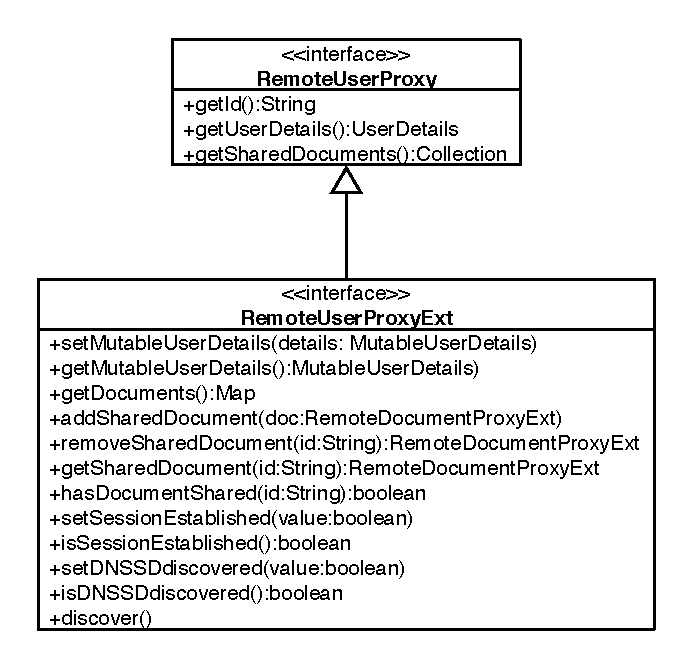
\includegraphics[width=4.40in,height=4.24in]{../images/finalreport/network_remoteUserProxyExt_uml.eps}
 }
 \caption{RemoteUserProxy and extension}
 \label{fig:network.discovery.remoteuserproxy.uml}
\end{figure}


\begin{figure}[H]
 \centering
  \frame{
 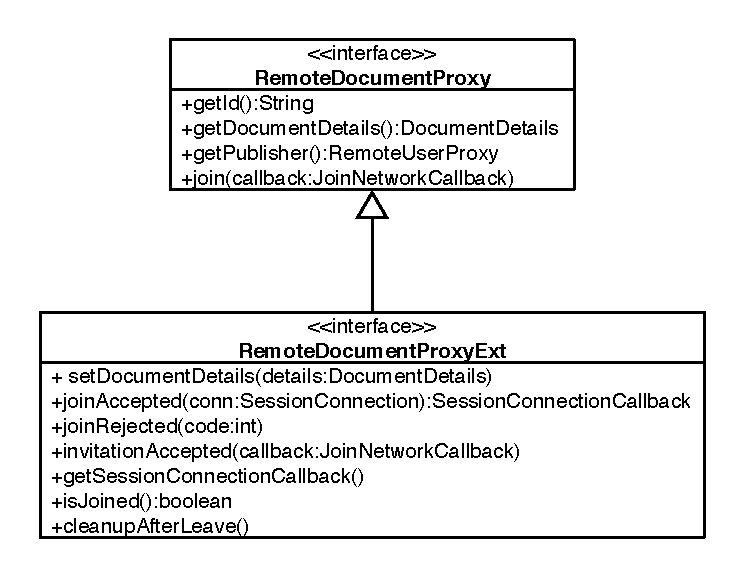
\includegraphics[width=4.99in,height=3.88in]{../images/finalreport/network_remoteDocumentProxyExt_uml.eps}
 }
 \caption{RemoteDocumentProxy and extension}
 \label{fig:network.discovery.remotedocumentproxy.uml}
\end{figure}

 \texttt{RemoteDocumentProxyExt} adds methods mainly for the join and invite use cases but also for updates of the document details. \emph{MutableUserDetails} contains the address and port information for the user. Method  \texttt{cleanupAfterLeave()} allows for a consistent object state since a document can be joined and left several times. So it is important to keep the object in one of two consistent states: \emph{Initialized} and \emph{Joined}.  

\begin{figure}[H]
 \centering
 \frame{
 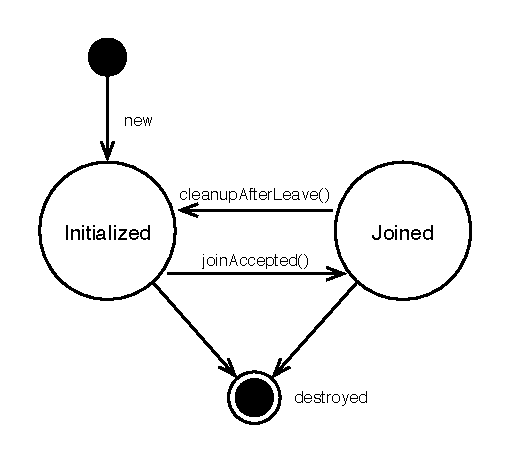
\includegraphics[width=3.18in,height=2.86in]{../images/finalreport/network_remoteDocumentProxy_state.eps}
 }
 \caption{RemoteDocumentProxy State Diagram}
 \label{fig:network.discovery.remotedocumentproxy.state}
\end{figure}

\subsubsection{Network Connection Management}
Network Connection Management includes the session and connection handling for each remote user. For each user, there is one \texttt{Remote\-User\-Session}. This class is a wrapper around \texttt{TCPSession} from the BEEP API and provides further session management functions. The \texttt{Session\-Manager} handles the creation and management of all \texttt{Remote\-User\-Session}s. For each session, there is one instance of \texttt{MainConnection}, through which most document management messages are sent to the respective peer. 

\begin{figure}[H]
 \centering
  \frame{
 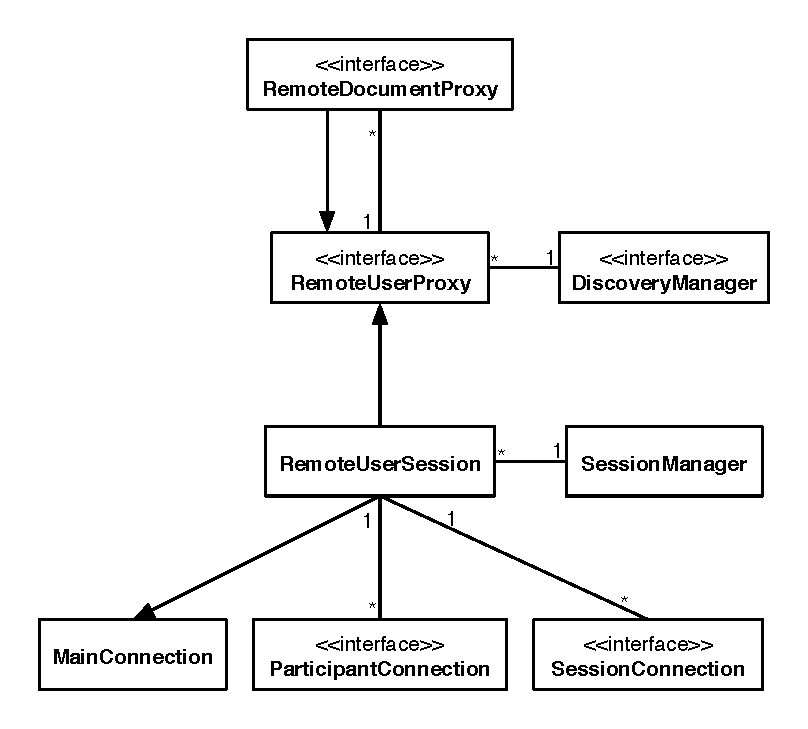
\includegraphics[width=5.17in,height=4.64in]{../images/finalreport/network_sessionManagement_uml.eps}
 }
 \caption{Session Management for a Remote User}
 \label{fig:network.discovery.sessionmanagement}
\end{figure}

Document management is considered to include the following messages:
\begin{itemize}
\item published document
\item concealed document
\item user invitation
\item user invitation rejected
\item join request
\item join request rejected
\item send published documents to discovered user
\item document details changed
\end{itemize}

Session management is considered to include the following messages:
\begin{itemize}
\item leave a document session
\item user kicked
\item document session terminated
\item operation request
\item caret update 
\item acknowledge
\item participant joined
\item participant left
\end{itemize}

Document management messages are sent via the \texttt{MainConnection} connection.

Session management messages are sent via the \texttt{ParticipantConnection} (publisher site) and the \texttt{SesssionConnection} (participant site), respectively. These connection types are explained next.

\paragraph{Connection types}
An \texttt{AbstractConnection} represents a physical connection to a peer. It is basically a wrapper around a \texttt{Channel} provided by the BEEP API. Implementations of \texttt{AbstractConnection} traverse several states during their lifetime. This is depicted in the following figure.

\begin{figure}[H]
 \centering
  \frame{
 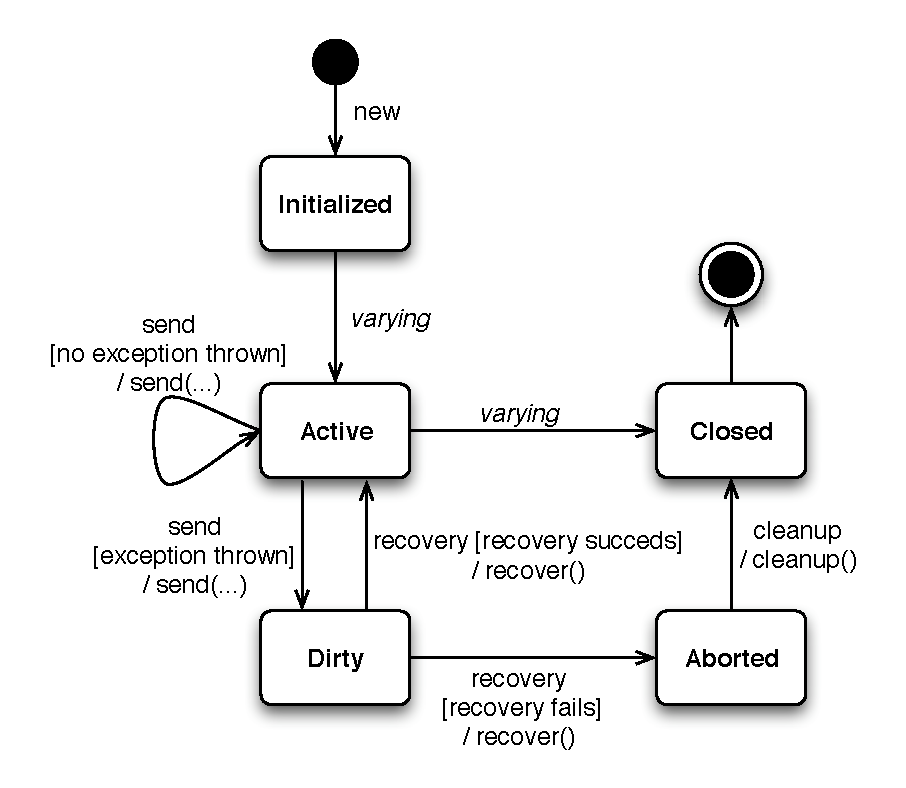
\includegraphics[width=5.82in,height=5.03in]{../images/finalreport/network_connection_state.eps}
 }
 \caption{State diagram for AbstractConnection}
 \label{fig:network.discovery.connection.state}
\end{figure}

The state transitions marked with \emph{varying} depend on the type of connection. The normal lifecycle would be the following states: \emph{initialized}, \emph{active} and \emph{closed}. Depending on whether a recovery mechanism is implemented, a connection may also turn into states \emph{dirty} and \emph{aborted}. If no recovery mechanism is implemented, the state directly becomes \emph{closed} when an exception occurs.

There are three different connection types which are shown in figure \ref{fig:network.protocol.connection.uml}.

\begin{figure}[H]
 \centering
  \frame{
 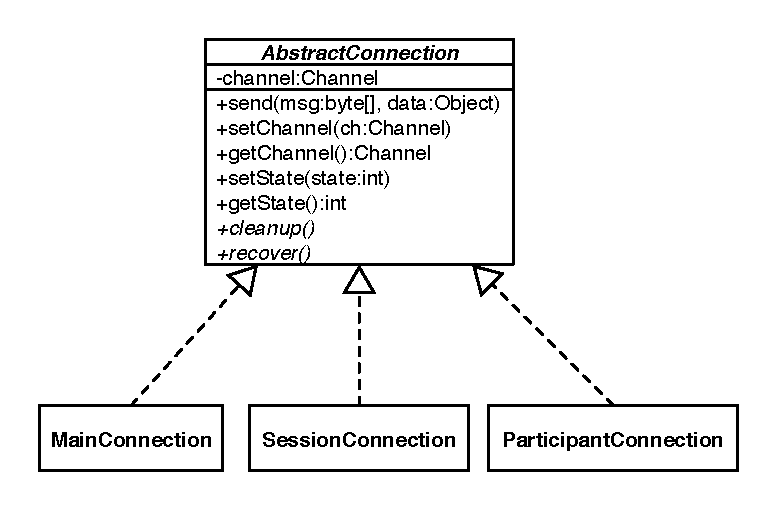
\includegraphics[width=4.96in,height=3.18in]{../images/finalreport/network_connection_uml.eps}
 }
 \caption{AbstractConnection Implementations}
 \label{fig:network.protocol.connection.uml}
\end{figure}


\subparagraph{MainConnection}
All basic communication messages (refered to as document management messages above) except the session messages are sent with the \texttt{MainConnection}. It wraps a BEEP channel which represents the physical connection to the peer. Each user has only one instance of \texttt{MainConnection} and therefore only one channel for the main communication. Both peers use that same physical channel bidirectionally to communicate with each other (this property is provided by the BEEP framework). The lifetime of the \texttt{MainConnection} endures for the lifetime of both users. If one user quits, the \texttt{MainConnection} is terminated too.

\subparagraph{SessionConnection}
The \texttt{SessionConnection} represents a physical connection starting from the local user to the session owner (publisher of document) in a collaborative editing session. Thus, \texttt{SessionConnection}'s are only used by participants and not by the owner of a session. It allows a particpant to send session relevant messages to the session owner. The lifetime is as long as the user participates in the document session or until the publisher of the document terminates the session.

\subparagraph{ParticipantConnection}
The \texttt{ParticipantConnection} represents a physical connection starting from the document session owner to a participant. Therefore, \texttt{ParticipantConnection}s are used only by session owners and not partcipants. It allows a session owner to send relevant messages to the participants. The liftetime of the \texttt{ParticipantConnection} is as long as the local user shares his document or until the participant quits its session membership. When a \texttt{ParticipantConnection} is initialized, it opens two channels to the peer. This is explained next.


\paragraph{Connection handling}
Connection management includes the connection architecture between peers. The BEEP API allows for many different variants. First, the most straightforward solution was to use one connection of type \texttt{MainConnection} for the document administration and one connection for each joined document session (\texttt{ParticipantConnection} or \texttt{SessionConnection}). The BEEP API allows to create an arbitrary number of connections and channels, respectively, from one \texttt{TCPSession} (wrapped by \texttt{RemoteUserSession}) and to use the channels bidirectionally, i.e. that both peers send and receive data concurrently and asynchronously. This was the approach that got implemented first based on the flexibilty and better performance argumentation. Due to unrecoverable and untrackable exceptions thrown from the BEEP framework at a high traffic rate (e.g. caused by two users in a session and both of them writing very fast which causes much network traffic), this solution had to be discarded and another solution to be found. 

The connection management design is depicted in figure \ref{fig:network.discovery.connection.architecture}.

\begin{figure}[H]
 \centering
  \frame{
 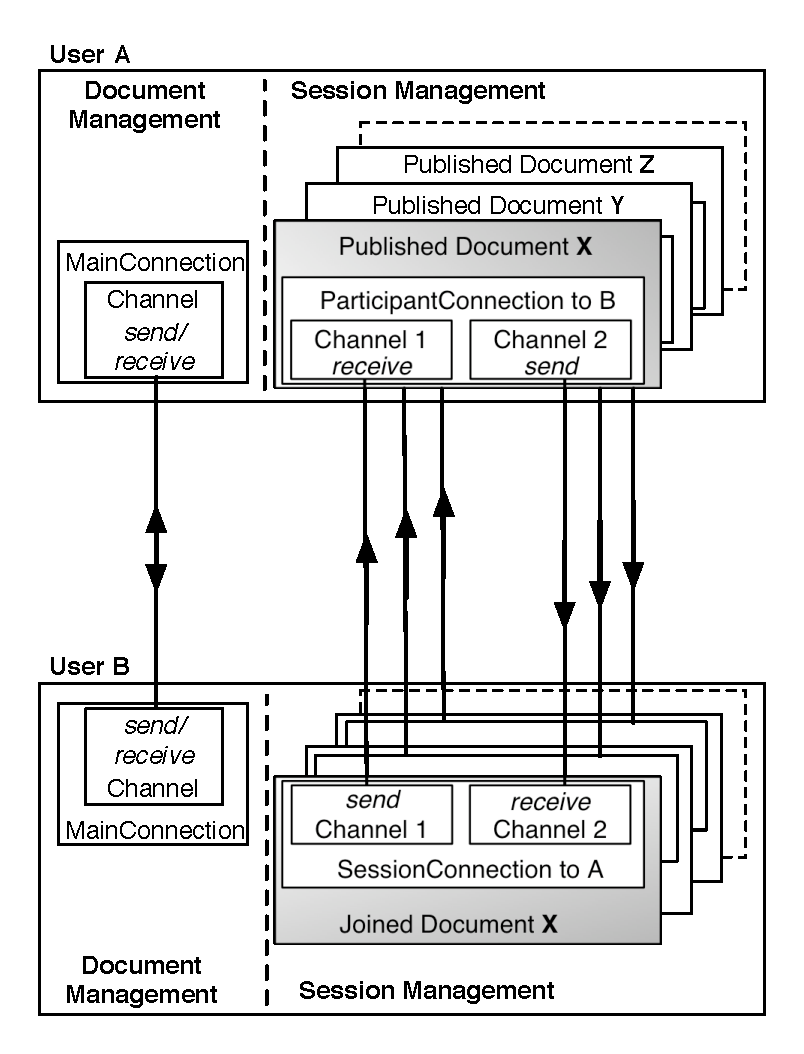
\includegraphics[width=5.14in,height=6.81in]{../images/finalreport/network_connection_architecture.eps}
 }
 \caption{Connection Architecture}
 \label{fig:network.discovery.connection.architecture}
\end{figure}


The \texttt{MainConnection} is used mostly for document management. This connection is used bidirectionally and asynchronously. Bidirectional means that messages are sent in both directions independently. Asynchronous means that the sender of a message does not wait until it gets a response from the recipient (a non-blocking asynchronous call). The traffic on the main connection gets never that high, so it has proved stable (as opposed to the session connections which broke on high traffic). There is always only one main connection between two peers independent of how many sessions a user is working on as depicted in figure \ref{fig:network.discovery.connection.architecture} with user A and user B.

For each session, the publisher has a \texttt{ParticipantConnection} to each of the participants (only user B in figure \ref{fig:network.discovery.connection.architecture}). Each \texttt{ParticipantConnection} has two channels with the peer. One channel is used to send messages and one channel is used to receive messages. Thus the transmission and the reception of messages can occur independently. At the server side (i.e. the user who published the document), one \texttt{ParticipantConnection} is created after both users agreed on collaborative editing in a particular document. The two channels are always initated within \texttt{ParticipantConnection} from the server side (user A) to the client side (user B) and never vice versa. Thus the client side (user B) 'receives' two channels from the server upon which it creates a \texttt{SessionConnection} to send and receive messages to and from user A, respectively.

For a precise understanding of the execution flow in establishing the session communication, compare the use case 'join document' in section \ref{chaper:protocol.usecases}.


\subsubsection{Network Message Processing}
Since the network layer implements a communication protocol, it must process outgoing (to the physical network) and incoming (from the physical network) messages. What could be a good design to fulfill this requirement? A solution is needed that is also flexible (i.e. easy adaptable to change) since an application procotol is often likely to change.

\paragraph{Message Filter Chain}
\label{chapter:network.protocol.messagefilterchain}
The concept for the processing of network messages is depicted in the following figure:

\begin{figure}[H]
 \centering
  \frame{
 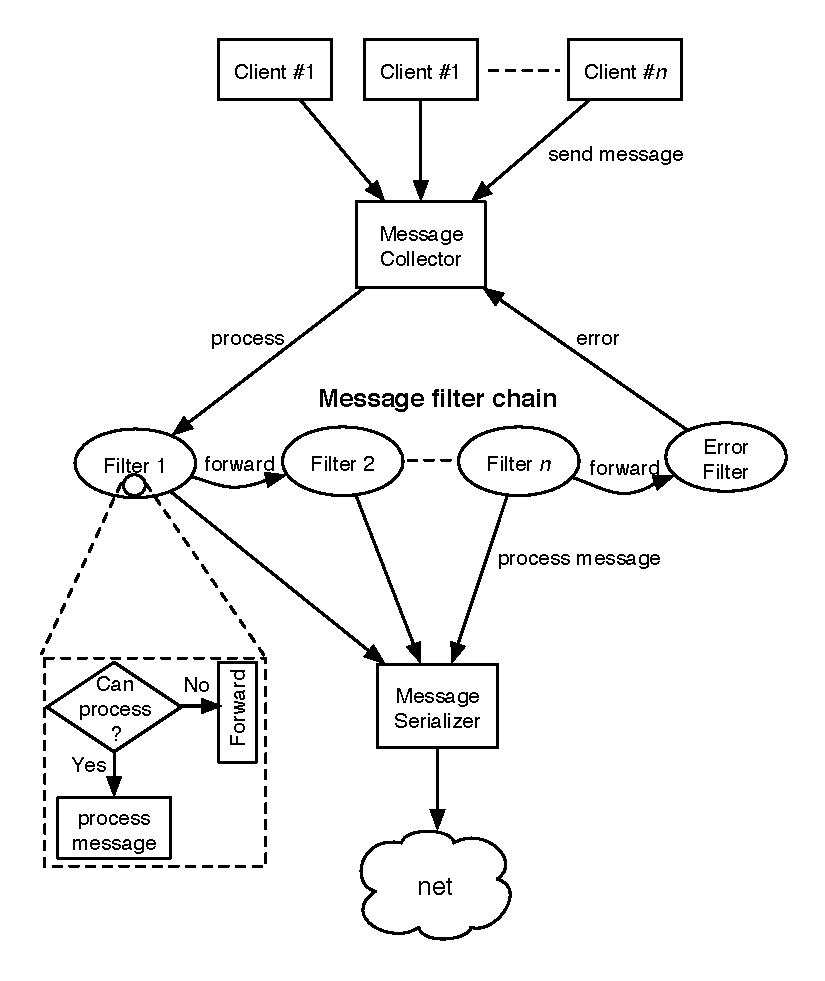
\includegraphics[width=5.28in,height=6.32in]{../images/finalreport/network_messageFilterChain_concept.eps}
 }
 \caption{Message Filter Chain}
 \label{fig:network.discovery.messagefilterchain.concept}
\end{figure}

Each message that needs to be processed is given to a \textbf{message filter chain}. The chaining of an arbitrary number of message filters with each one having one successor is dynamic and extensible. Each filter knows the exact message type it can process. If such a message arrives, it is processed by that filter and the algorithm stops. Otherwise, the message is forwarded to the successor. This happens repeatedly until a filter can process the message and then stops the forwarding. If no filter can process the message, it finally arrives at the last filter, a failure filter, which reports the failure to the client which initiated the message. If synchronization problems arose, a \texttt{ThreadDomain} could be prepended to the message filter chain to ensure proper synchronization.

If a new protocol message must be implemented, to accomplish the processing for that message only a new message filter must be added to the filter chain. And this could even be done at runtime. Therefore, the message filter chain allows for a dynamic composition of the protocol at runtime.

The concept of a message filter chain works for outgoing messages equally well as for incoming messages from the network (cf. the implementation section \ref{chapter:networkfilterchains}). 

A message filter is defined by the \texttt{RequestFilter} interface. The abstract super class \texttt{Abstract\-Request\-Filter} defines the common behavior for all message filters.

\begin{figure}[H]
 \centering
  \frame{
 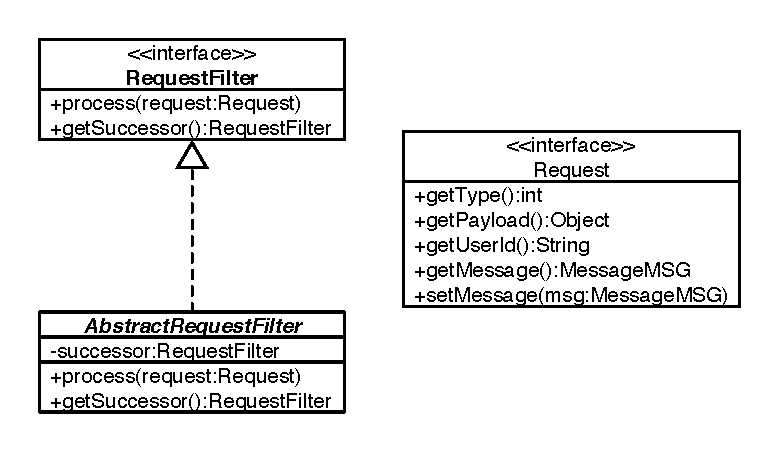
\includegraphics[width=4.97in,height=2.79in]{../images/finalreport/network_requestFilter_uml.eps}
 }
 \caption{Abstract Request Filter}
 \label{fig:network.discovery.abstractrequestfilter.uml}
\end{figure}


Each implementation of \texttt{AbstractRequestFilter} will have the following code structure inside its \texttt{process} method:

\begin{verbatim}
public void process(Request request) {
       if (request.getType() == MY_TYPE) {
             //process request...
       } else { 
             //forward request
             super.process(request);
       }
}
\end{verbatim}

See section \ref{network.communication.implementation} for the concrete implementation of this concept.

\newpage
\subsection{Implementation}
 \label{network.communication.implementation}

This section explains how the network layer was actually implemented. Its structure is oriented at the categorized requirements listing at the beginning of this chaper.

\subsubsection{NetworkService}
The central interface for the local user (i.e. the upper layer) but also for the network layer itself is \texttt{NetworkService} with an extension as shown in figure \ref{fig:network.discovery.networkservice.uml}.

\begin{figure}[H]
 \centering
  \frame{
 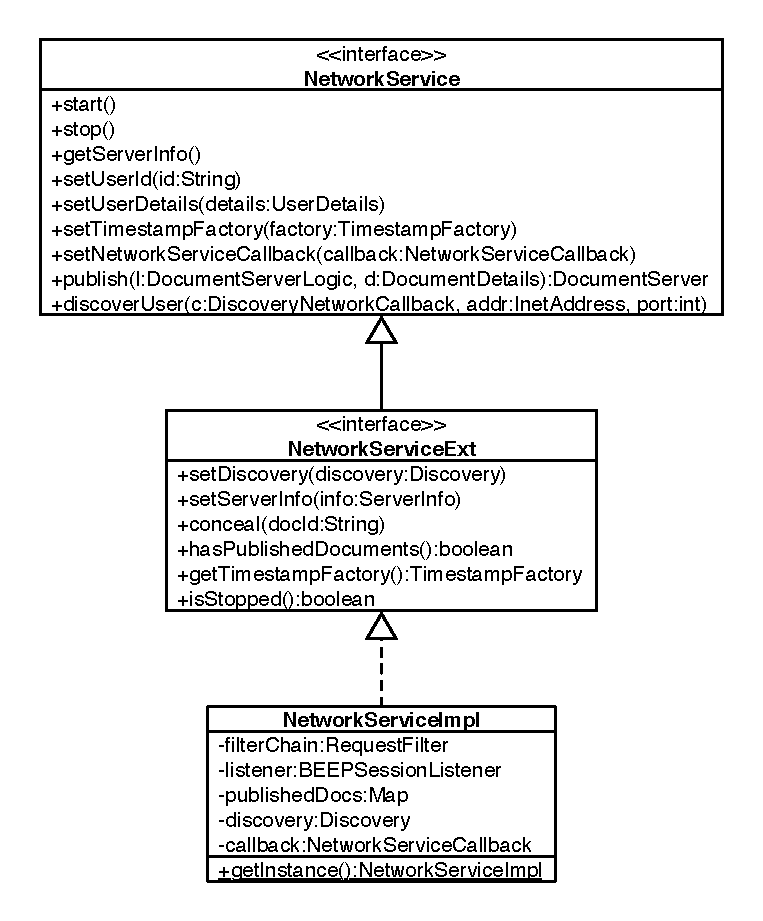
\includegraphics[width=4.86in,height=5.92in]{../images/finalreport/network_networkService_uml.eps}
 }
 \caption{Network Service with extension}
 \label{fig:network.discovery.networkservice.uml}
\end{figure}

The \texttt{NetworkService} is the main entry point for the upper layer. It provides basic functionality such as the start and stop of the network layer as well as the possibility to publish a document or to explicitly discover a user. The network layer itself works with type \texttt{NetworkServiceExt} which adds more methods for network layer level document management.

The implementation is a singleton instance since there exists only one network service per user and it is used many times in the network layer. On creation of the instance, the request filter chain (see below) and multiple factories are created.

The \texttt{NetworkService} receives a callback object of type \texttt{NetworkServiceCallback} to notify the upper layer about events on the network layer. The callback object is the main communication facility to the upper layer.


\subsubsection{Published Documents Management}
Published document management means the handling for all published documents of the local user. The network layer takes on server functionality with each published document. That is, it accepts join requests for the document and initiates the session communcation to agreed participants. Otherwise the network layer acts as a a client to other peers, e.g. it asks another peer to join a shared document. 

The notion of a published document is represented by the class \texttt{PublishedDocument}.

\begin{figure}[H]
 \centering
  \frame{
 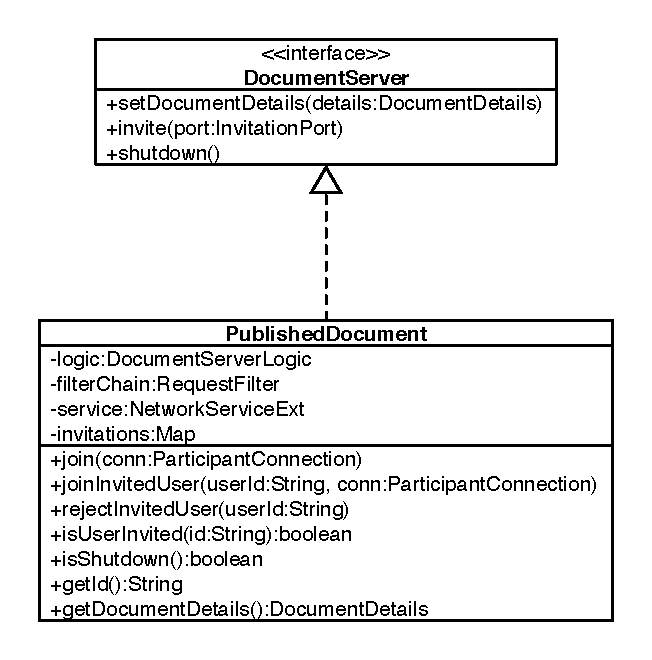
\includegraphics[width=4.12in,height=4.18in]{../images/finalreport/network_publishedDocument_uml.eps}
 }
 \caption{Published Document}
 \label{fig:network.discovery.publisheddocument.uml}
\end{figure}

The \texttt{PublishedDocument} implements the interface \texttt{DocumentServer} through which the upper layer communicates for the shared document (change document details, invite a user or shut down i.e. conceal the shared document).

The local user publishes a new document through the \texttt{publish} method of the \texttt{NetworkService}. There, a new instance of \texttt{PublishedDocument} is created. Additionally, the event of a new published document is communicated to all available peer users by means of the request filter chain which actually executes that task (i.e. the responsible filter, read \ref{chapter:networkfilterchains} for more on that).

The \texttt{PublishedDocument} provides methods so that the local user can invite other users to join that document or to process join requests from other users. The join requests are forwarded to the upper layer (i.e. \texttt{DocumentServerLogic}). 

When the published document is shut down, a conceal document message is sent to all available users and the resources for that published document released.

Thus far, we have considered the following architecture for publishing documents:
\begin{figure}[H]
 \centering
  \frame{
 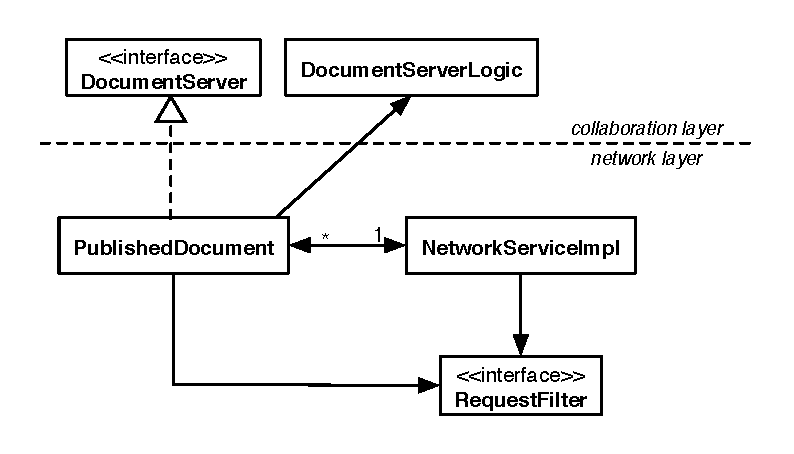
\includegraphics[width=5.07in,height=2.81in]{../images/finalreport/network_architecture1_uml.eps}
 }
 \caption{Architecture for \texttt{PublishedDocument}}
 \label{fig:network.protocol.architecture1.uml}
\end{figure}


\subsubsection{Remote User and Shared Documents Management}
The implementations of \texttt{RemoteUserProxy} and  \texttt{RemoteDocumentProxy} are as follows:

\begin{figure}[H]
 \centering
  \frame{
 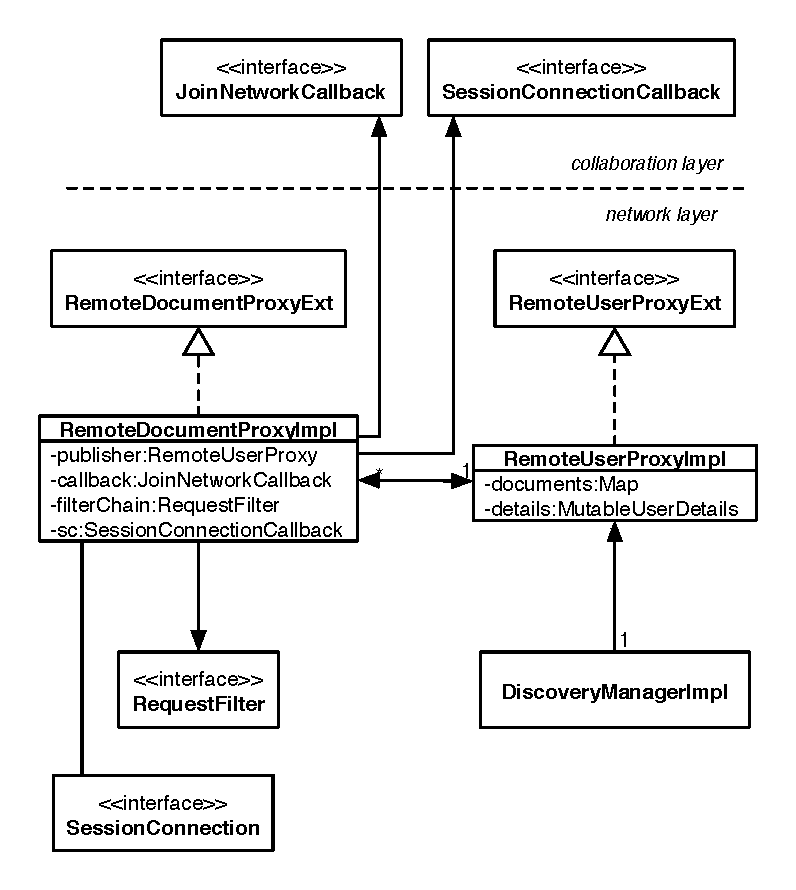
\includegraphics[width=5.08in,height=5.71in]{../images/finalreport/network_userImpl_uml.eps}
 }
 \caption{Imlementation of \texttt{RemoteUserProxy} and \texttt{RemoteDocumentProxy}}
 \label{fig:network.protocol.userimpl.uml}
\end{figure}

The \texttt{RemoteUserProxyImpl} class is straightforward. Each object is stored in the \texttt{DiscoveryManager} implementation. The \texttt{RemoteDocumentProxyImpl} class has two important references: one to an instance of type \texttt{JoinNetworkCallback} and one to an instance of type \texttt{SessionConnectionCallback}. 

The \texttt{JoinNetworkCallback} object is used to report the result of a request by the local user to join this document (call to method \texttt{join}). When the local user wants to \texttt{join} a document, a \texttt{Request} object is created and passed to the \texttt{RequestFilter} chain for processing. The result can be either \texttt{accepted} or \texttt{rejected}.

When the result of the join request is  \texttt{accepted}, the \texttt{JoinNetworkCallback} returns a \texttt{Session\-Connection\-Callback} object. This is the main communication port for a joined session to pass received messages to the upper layer (such as operations, caret updates, etc.).


\subsubsection{Session and Network Connection Management}
All connections for a particular remote user are created, maintained and released in the \texttt{RemoteUserSession} object (compare figure \ref{fig:network.discovery.sessionmanagement}). Note: the notion of a network message and a network request are used interchangeably except where explicitly defined differently.

Following, the lifecycle of each connection type is explained in greater detail.

\paragraph{MainConnection}
The \texttt{MainConnection} to a user is created when he is (explicitly) discovered. When discovery of a user happens, the main connection must be established in order to send the published documents of the local user to that remote user. If no published documents are available, the \texttt{MainConnection} is not established between the two peers until one user publishes a document. Once established, the main connection remains so for the whole application lifetime. Considering the state diagram \ref{fig:network.discovery.connection.state}, the \texttt{MainConnection} only passes through the following states: \texttt{active} and \texttt{closed}. When the object is created, the channel is already available and the connection directly goes to state  \texttt{active}. The \texttt{dirty} state is not yet possible since no recovery mechanism is implemented. If an exception occurs, the connection is closed.

\begin{figure}[H]
 \centering
  \frame{
 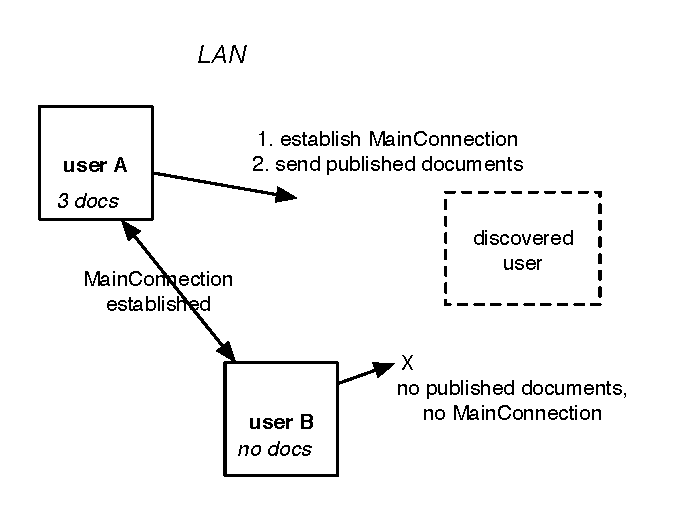
\includegraphics[width=4.31in,height=3.21in]{../images/finalreport/network_mainConnectionSetup.eps}
 }
 \caption{\texttt{MainConnection} setup only if published documents available}
 \label{fig:network.protocol.mainconnectionsetup}
\end{figure}

The idea behind this proceeding is that the new user does not have to ask all other users for their published documents and may get an empty response most of the time. It is better if users who have published documents send them to the new user, i.e. initiate the connection and push their document information to him. Thus, the system has less unnecessary communication in the sense that connections are only established if information to share is available.

\subparagraph{ParticipantConnection}
The implementation of \texttt{ParticipantConnection} is depicted in the following figure:

\begin{figure}[H]
 \centering
  \frame{
 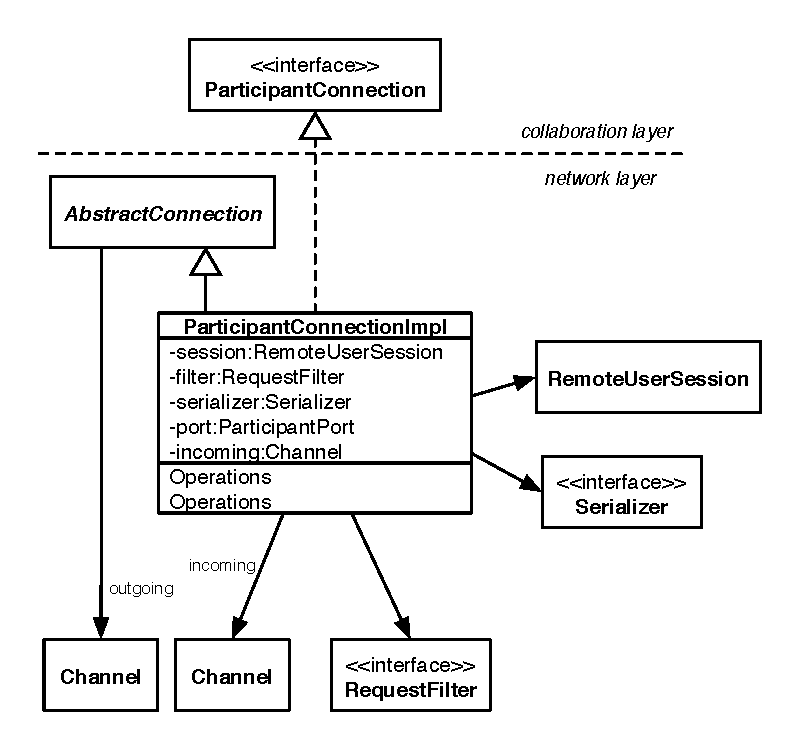
\includegraphics[width=5.11in,height=4.78in]{../images/finalreport/network_participantConnectionImpl_uml.eps}
 }
 \caption{\texttt{ParticipantConnection} Imlementation}
 \label{fig:network.protocol.participantconnectionimpl.uml}
\end{figure}

The \texttt{ParticipantConnection} is used by the upper layer to send messages to a peer. \texttt{Participant\-Connection\-Impl} serializes all messages using the \texttt{Serializer} and sends them to the peer with the outgoing channel. The sending of messages takes place in a synchronous mode, i.e. the sender waits for the response from the peer before it continues with the next message. This allows for more stability and easier synchronization but has a performance implication. However, the BEEP framework failed somehow using the asynchronous mode, so we were forced to go with synchronous session communication.

In order to receive messages from the network (through BEEP), each channel must be set a \texttt{RequestHandler} (see 'Processing of network messages' below for further details).

Consider the following figure:

\begin{figure}[H]
 \centering
  \frame{
 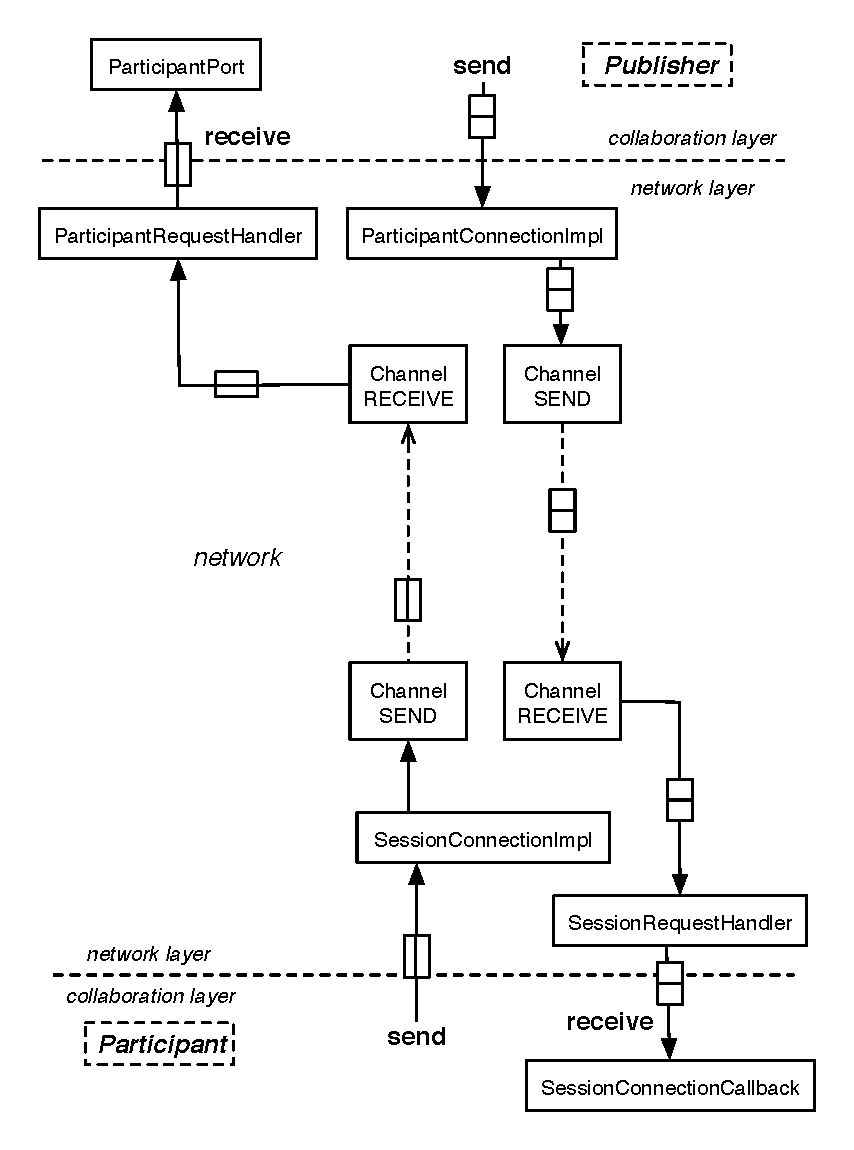
\includegraphics[width=5.47in,height=7.44in]{../images/finalreport/network_requestCommunication.eps}
 }
 \caption{Session Communication between to peers}
 \label{fig:network.protocol.requestcommunication}
\end{figure}

It shows the network message flow between the publisher and a participant in a document session using two \texttt{Channel}'s. The publisher sends its messages via the \texttt{ParticipantConnectionImpl} which has a channel that actually transmits the message. At the participant site, the messages are received and processed via the \texttt{Session\-Request\-Handler} and finally forwarded to the \texttt{Session\-Connection\-Callback}, i.e. the upper layer. In the other direction, the participant's messages are sent via the \texttt{SessionConnectionImpl} which uses a second channel to transmit them. At the publisher's site, the messages are received and processed by the \texttt{ParticipantRequestHandler} and finally forwarded to the \texttt{ParticipantPort}, which means the upper layer.

Considering the state diagram \ref{fig:network.discovery.connection.state}, the \texttt{ParticipantConnectionImpl} connection passes through the following states: \texttt{initialized}, \texttt{active} and \texttt{closed}. The \texttt{dirty} state is not yet possible since no recovery mechanism is implemented. If an exception occurs, the connection is closed, its resources released and a new one must be set up.

\subparagraph{SessionConnection}
The class \texttt{SessionConnectionImpl} is a straightforward extension and implementation of \texttt{AbstractConnection} and \texttt{SessionConnection}, respectively. Depending on the method invoked, it generates and serializes the appropriate message and transmits it to the peer via its \texttt{Channel} object.

As shown in figure \ref{fig:network.protocol.requestcommunication}, the \texttt{SessionConnectionImpl} is used at the participant site for session communication.

Considering the state diagram \ref{fig:network.discovery.connection.state}, the \texttt{SessionConnectionImpl} connection passes through the following states: \texttt{initialized}, \texttt{active} and \texttt{closed}. The \texttt{dirty} state is not yet possible since no recovery mechanism is implemented. If an exception occurs, the connection is closed, its resources released and a new one must be set up, i.e. the document session must be established again with that user.

\subsubsection{Network Message Processing}
In order to receive messages, a \texttt{RequestHandler} can be set on each channel (see also section \ref{chapter:framework.beepcore} on BEEP). A request handler takes over the task of parsing the message and processing it appropriately. Since there are multiple connection types and thus different sets of messages, there are also multiple implementations of the \texttt{RequestHandler} interface:

\begin{itemize}
 \item \texttt{MainRequestHandler} for the  \texttt{MainConnection} connection
 \item \texttt{ParticipantRequestHandler} for the \texttt{ParticipantConnectionImpl} connection
 \item \texttt{SessionRequestHandler} for the \texttt{SessionConnectionImpl} connection
\end{itemize}

Figure \ref{fig:network.protocol.requesthandler.uml} depicts the \texttt{RequestHandler} hierarchy.

\begin{figure}[H]
 \centering
  \frame{
 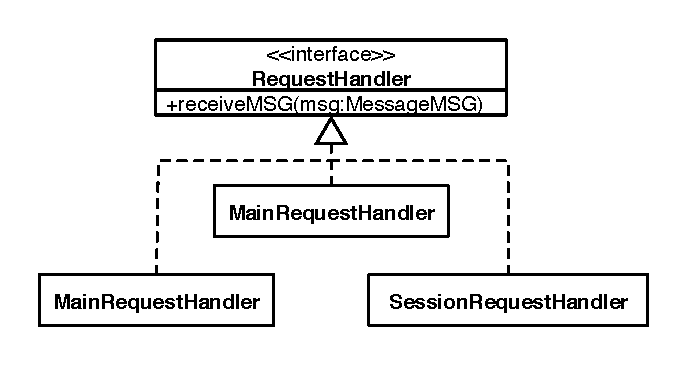
\includegraphics[width=4.36in,height=2.21in]{../images/finalreport/network_requestHandler_uml.eps}
 }
 \caption{\texttt{RequestHandler} Hierarchy}
 \label{fig:network.protocol.requesthandler.uml}
\end{figure}

Each implementation uses a \texttt{Deserializer} to parse the message and request, respectively (cf. section \ref{chapter:network.communication.protocol}). Afterwards, the request is processed according to its type. The \texttt{MainConnection} simply forwards the request to the request filter chain (see next section). The two other implementations know exactly what to do with a request and notify their recipient as shown in figure \ref{fig:network.protocol.requestcommunication}.

The \texttt{ParticipantRequestHandler} and the \texttt{SessionRequestHandler} are wrapped with a \texttt{SingleThreadDomain} to ensure proper synchronization, i.e. to have only one thread executing the \texttt{receiveMSG} method at a time. For each \texttt{ParticipantConnection} and \texttt{SessionConnection}, there exists one instance of \texttt{ParticipantRequestHandler} and \texttt{SessionRequestHandler}, respectively. Note that only one instance of \texttt{MainRequestHandler} is used as the request handler for all \texttt{MainConnection}'s as depicted in figure \ref{fig:network.protocol.requestfilterchain} .


\paragraph{Request Filter Chains}
\label{chapter:networkfilterchains}

The \texttt{RequestFilter} chain applies the message filter chain concept explained in section \ref{chapter:network.protocol.messagefilterchain}. The chain is put together according to the possible protocol messages. There exist two different request filter chains: 

\begin{itemize}
 \item A client chain for the processing of outgoing requests, ie. requests to be sent to peers
 \item A server chain for the processing of incoming requests, i.e. requests received from peers
\end{itemize}

These two constructs are shown in the following diagram:

\begin{figure}[H]
 \centering
  \frame{
 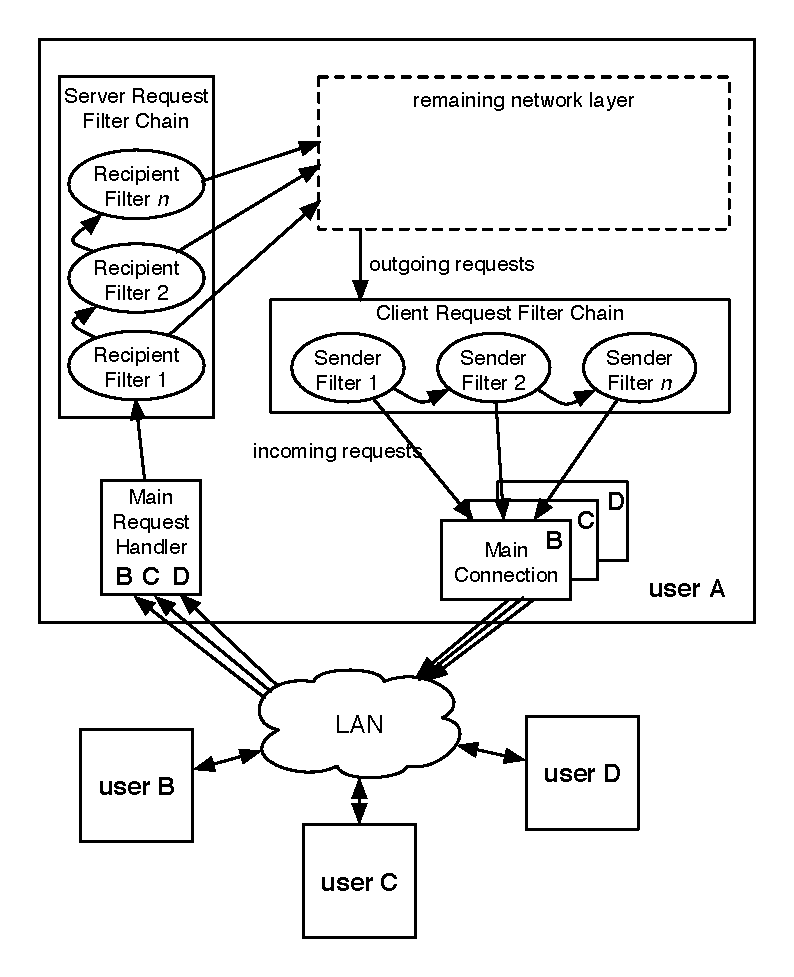
\includegraphics[width=5.07in,height=6.29in]{../images/finalreport/network_requestFilterChain.eps}
 }
 \caption{The client and server request filter chains}
 \label{fig:network.protocol.requestfilterchain}
\end{figure}

The picture shows a situation with four users A, B, C and D, respectively, in the same local area network. User A has three \texttt{MainConnection} established, one to each user B, C, and D. All \texttt{MainConnection}'s have the same \texttt{MainRequestHandler} set, i.e. all messages received from the three \texttt{MainConnection}s are processed by one \texttt{MainRequestHandler} object as depicted in the figure. \\
Each outgoing message is processed through the client request filter chain. Depending on the receiver of the request, the \texttt{MainConnection} object for user B, C, or D is used to send the request. When a message is received at user A, let's say from user B, it is deserialized by the \texttt{MainRequestHandler} object and then passed to the server request filter chain for further processing. Though there are multiple main connections, there is always only one client request filter chain and only one server request filter chain. The messages carry essential metadata. For example, the userid of the receiver of the message. This enables the sender filter responsible for handling the request to choose the correct \texttt{MainConnection} via the users' \texttt{RemoteUserSession}.

It would be possible to create a filter chain for response messages too (for a classical request-response communication), but this is currently not needed due to the protocol definition (cf. section 'Protocol'). The protocol currently defines only messages for asynchronous communication, i.e. a message is sent as a request but the response not immediately expected. Thus the response is sent back asynchronously, not in direct reply to the request. Thus it is considered a notification message meaning that the request has been processed and delivering its results.

Usually each message type has its own filter implementation. One filter for the creation of the message (added to the client chain) and one filter for the processing of the message (added to the server chain). For example, \texttt{JoinRequestSenderFilter} to send a join request and \texttt{JoinRequestRecipientFilter} to process a received join request (compare class \texttt{RequestFilterFactory}).


\subsubsection{Explicit User Discovery}
\label{chapter:network.protocol.explicituserdiscovery}
If an explicit user discovery needs to be executed, the method \texttt{discover()} on the respective \texttt{RemoteUserProxyExt} must be called. This method tries to establish a \texttt{RemoteUserSession} and \texttt{TCPSession}, respectively, with the given IP address and port. If this succeeds, a \texttt{MainConnection} is opened to that user and his metadata fetched. However, the upper layer is finally notified about the results of the discovery.



\subsection{Protocol}
\label{chapter:network.communication.protocol}
\subsubsection{Decision on data description language}
The first decision to be made was the kind of data description language to use. Two options were considered: XML or ASN.1/TLV. We considered that ASN.1 (Abstract Syntax Notation number One) in combination with TLV (Tag-Length-Value encoding) would be a reliable and high performance solution for the definition, encoding and decoding of the ACE protocol. Compared to XML, TLV needs few metata too to describe the messages and we considered that decoding with TLV would be faster than parsing XML. However, this considerations were abruptly abandonned by the fact that no mature open-source and free Java implementation for ASN.1/TLV exists to date. Nevertheless we found a library (see references) called the Apache ASN.1 Subproject. Its development version is 0.3 and currently undergoes a major refactoring. Also, it has few (Java) documentation and yet no Java parser for ASN.1 protocol definitions. So we decided that the risk for failure would be too high to actually try implementing the protocol with the Apache ASN.1 Subproject library and agreed on using XML for the protocol. Note: with XML we also have a platform and programming language independent data description language.

For the parsing of XML, we decided to use JAXP with SAX. Though the protocol defines many small messages, parsing is still faster with SAX than using JDom for example. Thus SAX is not only sufficient for our purpose but also considered more performant in parsing the messages.

Nevertheless, TLV is used beside XML for the document content encoding/decoding as explained below.

\subsubsection{Design}
There are five types of messages:

\begin{itemize}
\item channel
\item request
\item response
\item notification
\item session
\end{itemize}

\paragraph{Channel message}
The channel message is the first message that gets sent over the wire to initialize the channel. The channel message contains the channel type, either 'main' or 'session'. With this information, the request handler for the channel can be correctly determined.

\paragraph{Request message}
Only two types of messages are considered as requests in the sense that one user requests something from another user. And these two types are the 'join request' (a user wants to join another user's document) and the 'invite request' (a user invites another user to join his document).

\paragraph{Response message}
Response messages are sent upon requests. This is at an explicit user discovery where the response contains the userid and the name of the discovered user. Further, there are response messages 'joinRejected' and 'inviteRejected', i.e. when a user rejects another user's join request and when a user rejects an invitation, respectively. Another response message is created when a user lets another user join his document and a document response message containing all document information is created and sent to the joining user.

\paragraph{Notification message}
Notification messages are sent on events where other users 'might be interested to get to know it'. This includes messages for events 'userDiscarded', 'publish a document', 'conceal a document', 'send my published documents to discovered user', 'user kicked', 'user left' and 'document details changed'.

\paragraph{Session message}
The type session message includes all messages that are sent between users in a document editing session. This includes messages of kind 'operation', 'caret update', 'participant joined', 'participant left', 'acknowledgement' and 'session terminated'.


\subsubsection{Implementation}
The protocol is defined with an XML schema so that messages can be validated. This could be useful in particular for third party developers that might communicate with ACE.

The XML schema can be found in the subdirectory \texttt{src/\-resources/\-ch/\-iserver/\-ace/\-net/\-protocol/\-protocol.xsd} of the project.

To serialize the XML messages, an interface \texttt{Serializer} with two implementations \texttt{SerializerImpl} and \texttt{CollaborationSerializer} is used. The \texttt{SerializerImpl} is for document administration messages whereas \texttt{CollaborationSerializer} is for document session messages.

For deserialization, \texttt{ParserHandler} implementations together with a \texttt{SAXParser} (wrapped in an implementation of interface \texttt{Deserializer}) are used. The implementations are \texttt{RequestParserHandler} for messages on the \texttt{MainConnection} (i.e. document administration) and \texttt{CollaborationParserHandler} for messages in a document session (used in classes \texttt{ParticipantRequestHandler} and \texttt{SessionRequestHandler}).


\paragraph{TLV encoding/decoding}
When a published document has to be sent to a peer, it needs to be encoded. Considering the structure of a \texttt{PortableDocument}, many information must be encoded if for instance a user joins a document after four other users have been collaboratively editing it for half an hour. Therefore TLV is used to encode and decode this information (cf. \texttt{TLVHandler}). Each fragment is encoded as follows: the participant id is used as the tag. The length is the length of the fragment's text and the value is the text itself. 

After encoding the document to TLV, the data is Base64 encoded and gzip-compressed. The final data is then sent to the peer.


\subsubsection{BEEP classes}
The following classes are BEEP specific and are needed for a running BEEP infrastructure:

\begin{itemize}
\item \texttt{BEEPSessionListener}		- 	Listens for new (TCP-) sessions initiated by peers
\item \texttt{StartChannelListenerImpl} 	-	Called when a channel starts or closed 
\item \texttt{DefaultProfile}				-	The default profile used to register with BEEP
\end{itemize}


\subsubsection{Exception handling}
\label{chapter:network.exceptionhandling}
The \texttt{NetworkServiceCallback} provides a method \texttt{serviceFailure} to report errors to the upper layer. If the network layer is unable to recover from an exception (e.g. connection broken), resources are released and the error reported via the \texttt{serviceFailure} method to the upper layer. It was considered that no reasonable recovery algorithm could be implemented for network failures related to BEEP Core. However, the connection must be explicitly reestablished in this case by the end user, e.g. join the document again.


\subsection{Use Cases}
\label{chaper:protocol.usecases}

\subsubsection{Join a document}
The following sequence diagram shows the execution flow in the network layer when a join request for a published document arrives. The deserialization is left out for simplicity.

\begin{figure}[htb]
 \centering
 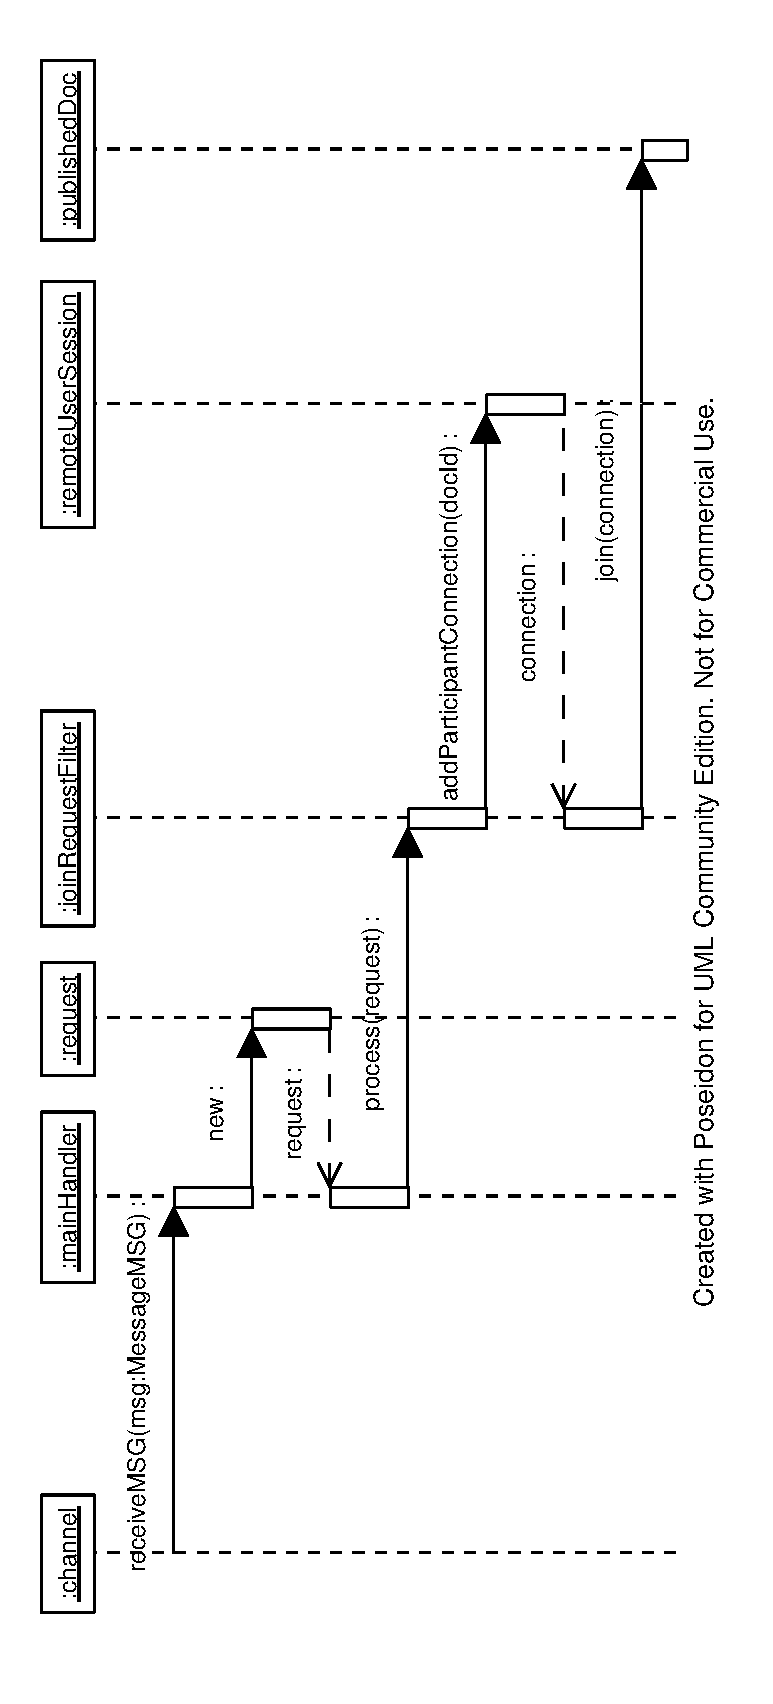
\includegraphics[width=7.07cm,height=16cm,angle=270]{../images/finalreport/network_joinRequest_sequence.eps}
 \caption{The processing of a join request at the publisher site}
 \label{fig:network.protocol.joinrequest}
\end{figure}

After calling \texttt{join} on the \texttt{PublishedDocument}, the local user will have to respond to the request. After the join request is granted, the collaboration layer invokes \texttt{joinAccepted} on the \texttt{ParticipantConnectionImpl}:


\begin{figure}[htb]
 \centering
 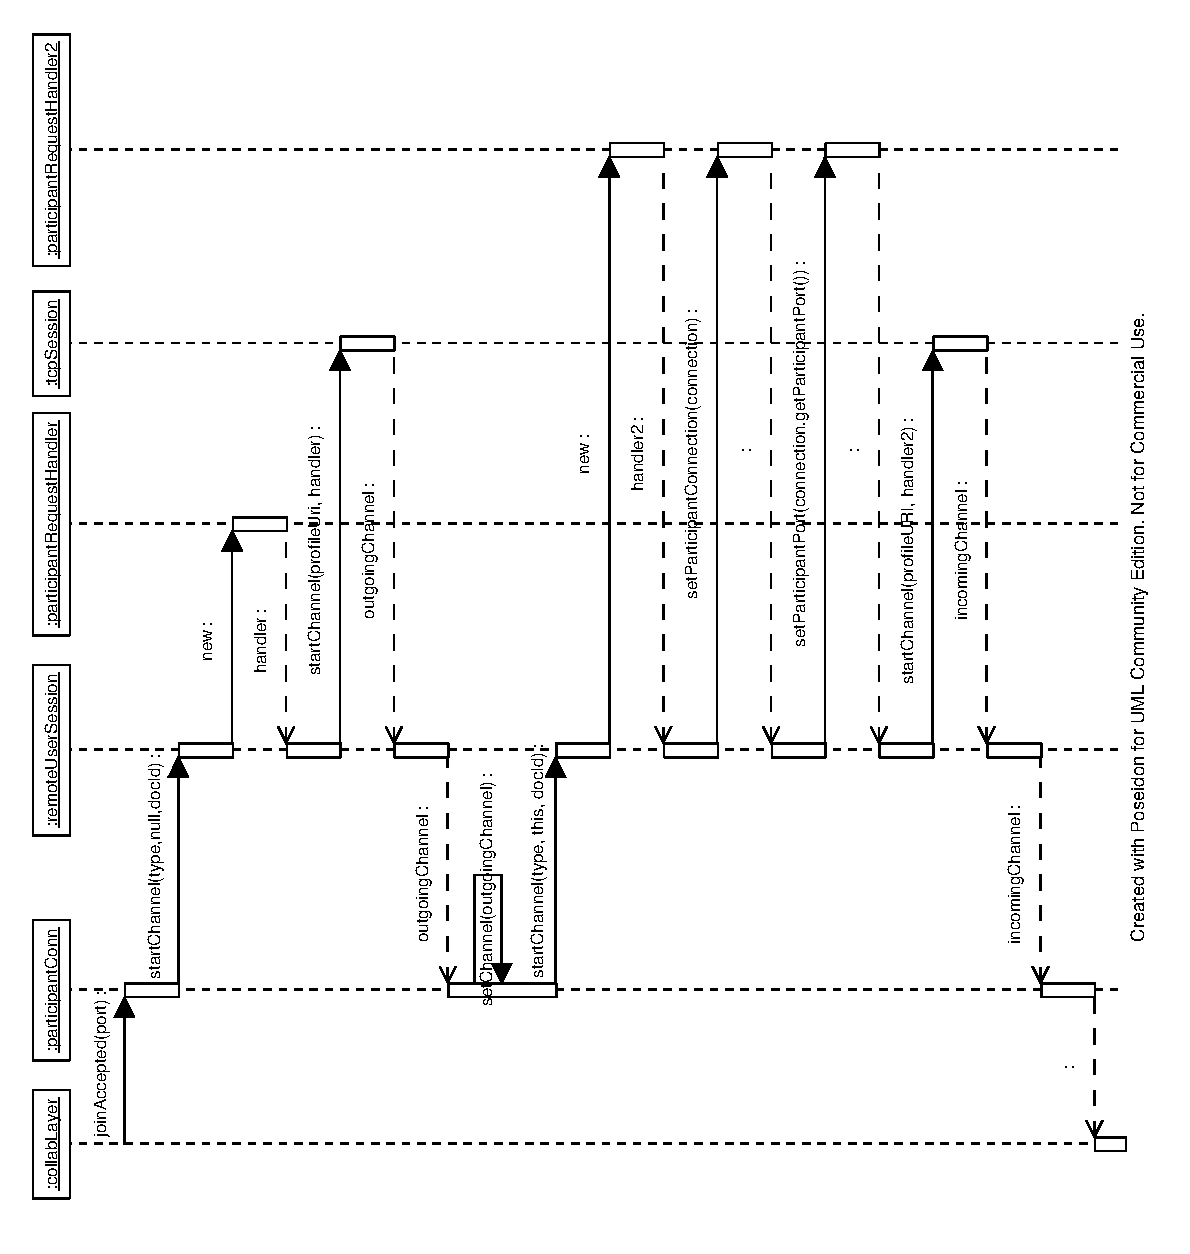
\includegraphics[width=14.67cm,height=16cm,angle=270]{../images/finalreport/network_joinRequest_sequence2.eps}
 \caption{The processing of a join request at publisher site after granting it}
 \label{fig:network.protocol.joinrequest2}
\end{figure}


Afterwards, the session connection between publisher and participant is established and ready to send the document content.



